% This is part of Mes notes de mathématique
% Copyright (c) 2008-2021
%   Laurent Claessens
% See the file fdl-1.3.txt for copying conditions.

%+++++++++++++++++++++++++++++++++++++++++++++++++++++++++++++++++++++++++++++++++++++++++++++++++++++++++++++++++++++++++++
\section{Intervalles}
%+++++++++++++++++++++++++++++++++++++++++++++++++++++++++++++++++++++++++++++++++++++++++++++++++++++++++++++++++++++++++++

\begin{definition}[Intervalle]
    Une partie \( I\) de \( \eR\) est un \defe{intervalle}{intervalle} si pour tout \( a,b\in I\) nous avons \( t\in I\) dès que \( a\leq t\leq b\).

    Un intervalle est \defe{ouvert}{intervalle!ouvert} s'il est de la forme \( \mathopen] a , b \mathclose[\) avec éventuellement \( a=-\infty\) ou \( b=+\infty\). Un intervalle est \defe{fermé}{intervalle!fermé} s'il est de la forme \( \mathopen[ a , b \mathclose]\) ou \( \mathopen] -\infty , b \mathclose]\) ou \( \mathopen[ a , +\infty [\) avec \( a,b\in \eR\).
\end{definition}

\begin{remark}
  L'ensemble $\eR$ ne contient pas $-\infty$ et $-\infty$. L'intervalle $[-\infty, 5]$ par exemple, n'est pas une partie de $\eR$.
\end{remark}

\begin{example}
    \begin{enumerate}
        \item
        Les ensembles \( \mathopen] 3 , 7 \mathclose[\) et \( \mathopen] -\infty , \pi \mathclose[\) sont des intervalles ouverts.
        \item
            Les ensembles \( \mathopen[ 10 , 15 \mathclose]\) et \( \mathopen[ -1 , +\infty [\) sont des intervalles fermés.
        \item
        L'ensemble \( \mathopen] -4 , -2 \mathclose[\cup\mathopen] 2 , 9 \mathclose[\) n'est pas un intervalle (il y a un «trou» entre \(- 2\) et \( 2\)).
        \item
            L'ensemble \( \eR\) lui-même est un intervalle; par convention, il est à la fois ouvert et fermé.
    \end{enumerate}
Un intervalle peut n'être ni ouvert ni fermé; par exemple \( \mathopen] 4 , 8 \mathclose]\). Cet intervalle est «ouvert en \( 4\) et fermé en \( 8\)» .
\end{example}

\begin{definition}[Fonction, domaine, image, graphe]
  Soient $X$ et $Y$ deux ensembles. Une \defe{fonction}{fonction} $f$ définie sur $X$ et à valeurs dans $Y$ est une correspondence qui associe à chaque élément $x$ dans $X$ {\bf au plus} un élément $y$ dans $Y$. On écrit $y= f(x)$.
  \begin{itemize}
  \item La partie de $X$ qui contient tous les $x$ sur lesquels $f$ peut opérer est dite \defe{domaine}{domaine} de $f$. Le domaine de $f$ est indiqué par $\Dom f$.
  \item L'élément de $y\in Y$ associé par $f$ à un élément $x\in \Dom f$ (c'est-à-dire $f(x) = y$)  est appellé \defe{image}{image} de $x$ par $f$. L'\defe{image}{fonction!image} de la fonction $f$ est la partie de $Y$ qui contient les images de tous les éléments de $\Dom f$. L'image de $f$ est indiquée par $\Im f$.
  \item Le \defe{graphe}{graphe} de $f$ est l'ensemble de toutes les couples $(x, f(x))$ pour $x\in \Dom f$. Le graphe de $f$ est une partie de l'ensemble noté $X\times Y$ et il est indiqué par $\Graph f$. Dans ce cours $X = \eR$ et $Y = \eR$, donc le graphe de $f$ est contenu dans le plan cartésien.
  \end{itemize}
\end{definition}

\begin{definition}[Fonction croissante, décroissante et monotone]
    Soit \( f\colon \eR\to \eR\) une fonction définie sur un intervalle \( I\subset \eR\).
    \begin{enumerate}
        \item
            Le fonction \( f\) est \defe{croissante}{fonction!croissante} sur \( I\) si pour tout \( x<y\) dans \( I\) nous avons \( f(x)\leq f(y)\). Elle est \emph{strictement} croissante si \( f(x)<f(y)\) dès que \( x<y\).
        \item
            Le fonction \( f\) est \defe{décroissante}{fonction!décroissante} sur \( I\) si pour tout \( x<y\) dans \( I\) nous avons \( f(x)\geq f(y)\). Elle est \emph{strictement} décroissante si \( f(x)>f(y)\) dès que \( x<y\).
        \item
            La fonction \( f\) est dite \defe{monotone}{fonction!monotone} sur \( I\) si elle est soit croissante soit décroissante sur \( I\).
    \end{enumerate}
\end{definition}

\begin{example}
    La fonction \( x\mapsto x^2\) est décroissante sur l'intervalle \( \mathopen] -\infty , 0 \mathclose]\) et croissante sur l'intervalle \( \mathopen[ 0 , \infty \mathclose[\). Elle n'est par contre ni croissante ni décroissante sur l'intervalle \( \mathopen[ -4 , 3 \mathclose]\).
\end{example}

%+++++++++++++++++++++++++++++++++++++++++++++++++++++++++++++++++++++++++++++++++++++++++++++++++++++++++++++++++++++++++++
\section{Application réciproque}
%+++++++++++++++++++++++++++++++++++++++++++++++++++++++++++++++++++++++++++++++++++++++++++++++++++++++++++++++++++++++++++

%---------------------------------------------------------------------------------------------------------------------------
\subsection{Définitions}
%---------------------------------------------------------------------------------------------------------------------------

Les définitions d'injection, surjection, bijection et d'application réciproque sont les définitions~\ref{DEFooBFCQooPyKvRK} et~\ref{DEFooTRGYooRxORpY}.

\begin{example}     \label{EXooCWYHooLEciVj}
    \begin{enumerate}
        \item
            La fonction \( x\mapsto x^2\) n'est pas une bijection de \( \eR\) vers \( \eR\) parce qu'il n'existe aucun \( x\) tel que \( x^2=-1\).
        \item
            La fonction
            \begin{equation}
                \begin{aligned}
                    f\colon \mathopen[ 0 , +\infty [&\to \mathopen[ 0 , +\infty [ \\
                    x&\mapsto x^2
                \end{aligned}
            \end{equation}
            est une bijection. Notez que c'est la même fonction que celle de l'exemple précédent. Seul l'intervalle sur laquelle nous nous plaçons a changé.
        \item
            La fonction
            \begin{equation}
                \begin{aligned}
                    f\colon \eR&\to \mathopen[ 0 , \infty \mathclose[ \\
                    x&\mapsto x^2
                \end{aligned}
            \end{equation}
            n'est pas une bijections parce qu'il existe plusieurs \( x\) pour lesquels \( f(x)=4\).
        \item
            Nous verrons un peu plus tard (\ref{PROPooXQYFooPxoEHE}) que l'application
            \begin{equation}
                \begin{aligned}
                    f\colon \mathopen[ 0 , \infty \mathclose[\to \mathopen[ 0 , \infty \mathclose[\\
                    x&\mapsto x^2
                \end{aligned}
            \end{equation}
            est une bijection.
    \end{enumerate}
    En conclusion : il est très important de préciser les domaines des fonctions considérées.
\end{example}

\begin{remark}
    Dire que la fonction \( f\colon I\to J\) est bijective, c'est dire que l'équation \( f(x)=y\) d'inconnue \( x\) peut être résolue de façon univoque pour tout \( y\in J\).
\end{remark}

\begin{remark}
  Toute fonction strictement monotone sur un intervalle $I$ est injective.
\end{remark}

\begin{example}
    Trouvons la fonction réciproque de la fonction affine \( f\colon \eR\to \eR\), \( x\mapsto 3x-2\). Si \( y\in \eR\) le nombre \( f^{-1}(y)\) est la valeur de \( x\) pour laquelle \( f(x)=y\). Il s'agit donc de résoudre
    \begin{equation}
        3x-2=y
    \end{equation}
    par rapport à \( x\). La solution est \( x=\frac{ y+2 }{ 3 }\) et donc nous écrivons
    \begin{equation}
        f^{-1}(y)=\frac{ y+2 }{ 3 }.
    \end{equation}
    Notons que dans les calculs, il est plus simple d'écrire «\( y\)» que «\( x\)» la variable de la fonction réciproque. Il est néanmoins (très) recommandé de nommer «\( x\)» la variable dans la réponse finale. Dans notre cas nous concluons donc
    \begin{equation}
        f^{-1}(x)=\frac{ x+2 }{ 3 }.
    \end{equation}
\end{example}

%---------------------------------------------------------------------------------------------------------------------------
\subsection{Graphe de la fonction réciproque}
%---------------------------------------------------------------------------------------------------------------------------

Par définition le graphe de la fonction \( f\) est l'ensemble des points de la forme \( (x,y)\) vérifiant \( y=f(x)\). Afin de déterminer le graphe de la bijection réciproque nous pouvons faire le raisonnement suivant.

        Le point \( (x_0,y_0)\) est sur le graphe de \( f\)

\noindent\( \Leftrightarrow\)

        La relation \( f(x_0)=y_0\) est vérifiée

\noindent\( \Leftrightarrow\)

        La relation \( x_0=f^{-1}(y_0)\) est vérifiée

\noindent\( \Leftrightarrow\)

        Le point \( (y_0,x_0)\) est sur le graphe de \( f^{-1}\).

\begin{Aretenir}
    Dans un repère orthonormal, le graphe de la bijection réciproque est obtenu à partir du graphe de \( f\) en effectuant une symétrie par rapport à la droite d'équation \( y=x\).
\end{Aretenir}

Le dessin suivant montre le cas de la courbe de la fonction carré comparé à celle de la racine carrée.
\begin{center}
   \input{auto/pictures_tex/Fig_CELooGVvzMc.pstricks}
\end{center}


%+++++++++++++++++++++++++++++++++++++++++++++++++++++++++++++++++++++++++++++++++++++++++++++++++++++++++++++++++++++++++++
\section{Topologie sur l'ensemble des réels}
%+++++++++++++++++++++++++++++++++++++++++++++++++++++++++++++++++++++++++++++++++++++++++++++++++++++++++++++++++++++++++++
\label{SECooGKHYooMwHQaD}

Nous allons à présent donner la topologie sur \( \eR\) et ainsi résoudre les questions laissées en suspens lors de la construction des réels, voir~\ref{NormooHRDZooRGGtCd}.


Afin de pouvoir étudier la topologie des espaces métriques, il faut savoir quelques propriétés des réels parce que nous allons étudier la fonction distance qui est une fonction continue à valeurs dans les réels.

La valeur absolue de la définition~\ref{DefKCGBooLRNdJf}\ref{ItemooWUGSooRSRvYC} permet de définir une norme sur \( \eR\).
\begin{lemma}       \label{LEMooBNAPooBTtXnX}
    L'application
    \begin{equation}
         x\mapsto | x |
    \end{equation}
    est une norme\footnote{Définition \ref{DefNorme}.} sur $\eR$.
\end{lemma}

\begin{proof}
  Grâce au lemme \ref{LemooANTJooYxQZDw} et à la remarque \ref{RemooJCAUooKkuglX}, on a, pour tous \(x,\ y,\ \lambda \in \eR \):
\begin{enumerate}
\item $| x |=0$ implique $x=0$,
\item $| \lambda x |=| \lambda | |x |$,
\item $| x+y |\leq | x |+| y |$,
\end{enumerate}
et donc, les conditions de la définition \ref{DefNorme} sont immédiatement vérifiées.
\end{proof}

\begin{definition}[Topologie sur \( \eR\) et sur \( \eQ\)]      \label{DEFooNYGIooVGHSIA}
    Le lemme \ref{LEMooBNAPooBTtXnX} donne une norme sur \( \eR\) et \( \eQ\) à partir de la valeur absolue. La définition \ref{ThoORdLYUu} donne alors une structure d'espace topologique. Hors cas rarissimes qui seront signalés, nous utiliserons toujours cette topologie sur \( \eR\) et sur \( \eQ\).

\end{definition}

\begin{proposition}     \label{PropooUHNZooOUYIkn}
    Les rationnels sont denses dans les réels\footnote{Pour les topologies usuelles données en la définition \ref{DEFooNYGIooVGHSIA}.}.
\end{proposition}
\index{densité!de \( \eQ\) dans \( \eR\)}

\begin{proof}
    Soient \( r\in \eR\) et \( \epsilon\in \eR^+\). Nous devons prouver l'existence d'un rationnel dans \( B(x,\epsilon)\). Le lemme~\ref{LemooHLHTooTyCZYL} dit qu'il existe un rationnel dans \( \mathopen] x-\epsilon/2 , x+\epsilon/2 \mathclose[\) et donc dans \( B(x,\epsilon)\).
\end{proof}

\begin{proposition}[\cite{MonCerveau}] \label{PropSLCUooUFgiSR}
    Quel que soit le réel \( r\), il existe une suite croissante de rationnels convergente vers \( r\).
\end{proposition}

\begin{proof}
    Soient \( x\in \eR\) et \( \delta\in \eR\); vu que \( x-\delta\) et \( x\) sont des réels, le lemme~\ref{LemooHLHTooTyCZYL} donne un élément \( x_{\delta}\in \eQ \) tel que
    \begin{equation}
        x-\delta<x_{\delta}<x.
    \end{equation}
    Il suffit alors de pêcher parmi ces \( x_{\delta}\) pour trouver une suite croissante, et on montrera que cette suite converge vers \( x \).

    Soit \( x_0\) un rationnel plus petit que \( x\). Nous posons \( \delta_0=x-x_0\) et ensuite :
    \begin{subequations}
        \begin{numcases}{}
            \delta_i=x-x_i\\
            x_{i+1}=x_{\delta_i/2} \in \eQ.
        \end{numcases}
    \end{subequations}
    Ainsi nous avons pour tout \( i\) les inégalités
    \begin{equation}
        x_i=x-\delta_i<x-\frac{ \delta_i }{ 2 }<x_{i+1}<x.
    \end{equation}
    La suite \( (x_i) \) est donc une suite de rationnels, croissante et toujours plus petite que \( x\). Mais nous avons à chaque étape \( \delta_{i+1}<\frac{ \delta_i }{ 2 }\), ce qui implique que la suite des  \( \delta_i \) converge vers \( 0 \). Soit \( \epsilon>0\). Il existe \( k_0\) tel que pour tout \( k > k_0 \), \( \delta_k<\epsilon\). Pour un tel \( k \), nous avons alors
    \begin{equation}
        x_{k+1}\in B(x,\frac{ \delta_k }{ 2 })\subset B(x,\epsilon).
    \end{equation}
Tous les \( x_k \), pour \( k > k_0 + 1 \), sont tels que \( |x - x_k| < \epsilon \): la suite des \( x_k \) converge donc vers \( x \).
\end{proof}

%--------------------------------------------------------------------------------------------------------------------------- 
\subsection{Compacité pour les réels}
%---------------------------------------------------------------------------------------------------------------------------

Pour la définition générale d'un compact, c'est \ref{DefJJVsEqs}.

\begin{proposition}     \label{PROPooBFSAooKSugMj}
    Les parties compactes de \( \eR\) sont fermées et bornées.
\end{proposition}

\begin{proof}
Prouvons d'abord qu'un ensemble compact est borné. Pour cela, supposons que $K$ est un compact non borné vers le haut\footnote{Nous laissons à titre d'exercice le cas où $K$ est borné par le haut et pas par le bas.}. Donc il existe une suite infinie de nombres strictement croissante $x_1<x_2<\ldots$ tels que $x_i\in K$. Prenons n'importe quel recouvrement ouvert de la partie de $K$ plus petite ou égale à $x_1$, et complétons ce recouvrement par les ouverts $\mO_i=]x_{i-1},x_i[$. Le tout forme bien un recouvrement de $K$ par des ouverts.

Il n'y a cependant pas moyen d'en tirer un sous recouvrement fini parce que si on ne prend qu'un nombre fini parmi les $\mO_i$, on en aura fatalement un maximum, disons $\mO_k$. Dans ce cas, les points $x_{k+1}$, $x_{k+1}$,\ldots ne seront pas dans le choix fini d'ouverts.

Cela prouve que $K$ doit être borné.

Pour prouver que $K$ est fermé, nous allons prouver que le complémentaire est ouvert. Et pour cela, nous allons prouver que si le complémentaire n'est pas ouvert, alors nous pouvons construire un recouvrement de $K$ dont on ne peut pas extraire de sous recouvrement fini.

Si $\eR\setminus K$ n'est pas ouvert, il possède un point, disons $x$, tel que tout voisinage de $x$ intersecte $K$. Soit $B(x,\epsilon_1)$, un de ces voisinages, et prenons $k_1\in K\cap B(x,\epsilon_1)$. Ensuite, nous prenons $\epsilon_2$ tel que $k_1$ n'est pas dans $B(x,\epsilon_1)$, et nous choisissons $k_2\in K\cap B(x,\epsilon_2)$. De cette manière, nous construisons une suite de $k_i\in K$ tous différents et de plus en plus proches de $x$. Prenons un recouvrement quelconque par des ouverts de la partie de $K$ qui n'est pas dans $B(x,\epsilon_1)$. Les nombres $k_i$ ne sont pas dans ce recouvrement.

Nous ajoutons à ce recouvrement les ensembles $\mO=]k_i,k_{i+1}[$. Le tout forme un recouvrement (infini) par des ouverts dont il n'y a pas moyen de tirer un sous recouvrement fini, pour exactement la même raison que la première fois.
\end{proof}

\begin{theorem}[Borel-Lebesgue]   \label{ThoBOrelLebesgue}
    Un intervalle de \( \eR\) est compact si et seulement si il est de la forme \( \mathopen[ a , b \mathclose]\).
\end{theorem}

\begin{proof}
    Tous les intervalles de \( \eR\) sont listés dans la proposition \ref{PROPooHPMWooQJXCAS}. Un compact est fermé et borné (proposition \ref{PROPooBFSAooKSugMj}). Donc les intervalles dont une borne est \( \pm\infty\) ne sont pas compacts. Parmi les intervalles \( \mathopen] a , b \mathclose[\), \( \mathopen] a , b \mathclose]\), \( \mathopen[ a , b \mathclose[\) et \( \mathopen[ a , b \mathclose]\), seul le dernier est fermé. Nous avons prouvé que si un intervalle est compact, alors il est de la forme \( \mathopen[ a , b \mathclose]\). 

    Nous prouvons à présent l'implication inverse : tous les intervalles de la forme \( \mathopen[ a , b \mathclose]\) sont compacts.

    Soit $\Omega$, un recouvrement du segment $[a,b]$ par des ouverts, c'est-à-dire que
    \begin{equation}
        [a,b]\subseteq\bigcup_{\mO\in\Omega}\mO.
    \end{equation}
    Nous notons par $M$ le sous-ensemble de $[a,b]$ des points $m$ tels que l'intervalle $[a,m]$ peut être recouvert par un sous-ensemble fini de $\Omega$. C'est-à-dire que $M$ est le sous-ensemble de $[a,b]$ sur lequel le théorème est vrai. Le but est maintenant de prouver que $M=[a,b]$.
    \begin{description}
        \item[$M$ est non vide] En effet, $a\in M$ parce que il existe un ouvert $\mO\in\Omega$ tel que $a\in\mO$. Donc $\mO$ tout seul recouvre l'intervalle $[a,a]$.
        \item[$M$ est un intervalle] Soient $m_1$, $m_2\in M$. Le but est de montrer que si $m'\in[m_1,m_2]$, alors $m'\in M$. Il y a un sous recouvrement fini de l'intervalle $[a,m_2]$ (par définition de $m_2\in M$). Ce sous recouvrement fini recouvre évidemment aussi $[a,m']$ parce que $[a,m']\subseteq [a,m_2]$, donc $m'\in M$.
        \item[$M$ est une ensemble ouvert] Soit $m\in M$. Le but est de prouver qu'il y a un ouvert autour de $m$ qui est contenu dans $M$. Mettons que $\Omega'$ soit un sous recouvrement fini qui contienne l'intervalle $[a,m]$. Dans ce cas, on a un ouvert $\mO\in\Omega'$ tel que $m\in\mO$. Tous les points de $\mO$ sont dans $M$, vu qu'ils sont tous recouverts par $\Omega'$. Donc $\mO$ est un voisinage de $m$ contenu dans $M$.
        \item[$M$ est un ensemble fermé] $M$ est un intervalle qui commence en $a$, en contenant $a$, et qui finit on ne sait pas encore où. Il est donc soit de la forme $[a,m]$, soit de la forme $[a,m[$. Nous allons montrer que $M$ est de la première forme en démontrant que $M$ contient son supremum $s$. Ce supremum est un élément de $[a,b]$, et donc il est contenu dans un des ouverts de $\Omega$. Disons $s\in\mO_s$. Soit $c$, un élément de $\mO_s$ strictement plus petit que $c$; étant donné que $s$ est supremum de $M$, cet élément $c$ est dans $M$, et donc on a un sous recouvrement fini $\Omega'$ qui recouvre $[a,c]$. Maintenant, le sous recouvrement constitué de $\Omega'$ et de $\mO_s$ est fini et recouvre $[a,s]$.
    \end{description}
    Nous pouvons maintenant conclure : le seul intervalle non vide de $[a,b]$ qui soit à la fois ouvert et fermé est $[a,b]$ lui-même (proposition \ref{PropHSjJcIr}), ce qui prouve que $M=[a,b]$, 
    et donc que $[a,b]$ est compact\footnote{Si vous n'aimez pas le coup du fermé et ouvert, le lemme \ref{LemOACGWxV} donne une autre preuve.}.
\end{proof}


\begin{lemma}[\cite{JUwQXOF}]\label{LemOACGWxV}
    Si \( a<b\in \eR\) alors le segment \( \mathopen[ a , b \mathclose]\) est compact\footnote{Définition~\ref{DefJJVsEqs}}.
\end{lemma}
\index{compact!intervalle \( \mathopen[ a , b \mathclose]\)}

\begin{proof}
    Soit \( \{ \mO_i \}_{i\in I}\) un recouvrement de \( \mathopen[ a , b \mathclose]\) par des ouverts. Nous posons
    \begin{equation}
        M=\{ x\in\mathopen[ a , b \mathclose]\tq \mathopen[ a , x \mathclose] \text{ admet un sous-recouvrement fini extrait de } \{ \mO_i \}_{i\in I} \}.
    \end{equation}
    Notre but est de prouver que \( b\in M\).
    \begin{subproof}

    \item[\( a\) est dans \( M\)]

        Le point \( a\) est naturellement dans un des \( \mO_i\). L'intervalle \( \mathopen[ a , a \mathclose]\) est donc recouvert par un seul des \( \mO_i\).

    \item[\( M\) est un intervalle]

        Soient \( m\in M\) et \( m'\in\mathopen[ a , m [\). Le sous-recouvrement fini qui recouvre \( \mathopen[ a , m \mathclose]\) recouvre a fortiori \( \mathopen[ a , m' \mathclose]\).

    \item[Les trois possibilités restantes]
        À ce niveau de la preuve, il reste trois possibilités pour \( M\) soit il est de la forme \( \mathopen[ a , c \mathclose]\) ou \( \mathopen[ a , c [\) avec \( c<b\), soit il est de la forme \( \mathopen[ a , b \mathclose]\). Nous allons maintenant éliminer les deux premiers cas.

    \item[Ce que \( M\) n'est pas]

        D'abord \( M\) n'est pas de la forme \( \mathopen[ a , c [\) avec \( c<b\). Par l'absurde, commençons par considérer \( \mO_{i_0}\) un ouvert du recouvrement qui contient \( c\); choisissons  \(m \in \mO_{i_0}\) tel que \( m<c\). Alors \( m \in M \), et, si nous joignons \( \mO_{i_0}\) à un recouvrement fini de \( \mathopen[ a , m \mathclose]\) alors nous avons un recouvrement fini de \( \mathopen[ a , c \mathclose]\). On en déduit \( c\in M\).

        Ensuite \( M\) n'est pas de la forme \( \mathopen[ a , c \mathclose]\) avec \( c<b\). En effet si on a un recouvrement fini de \( \mathopen[ a , c \mathclose]\) par des ouverts, alors un de ces ouverts contient \( c\) et donc contient des éléments de \( \mathopen[ a , b \mathclose]\) plus grands que \( c\).
    \end{subproof}
    Nous déduisons que \( M=\mathopen[ a , b \mathclose]\) et qu'il est possible d'extraire un sous-recouvrement fini recouvrant \( \mathopen[ a , b \mathclose]\).
\end{proof}

\begin{lemma}[\cite{MonCerveau}]\label{LemCKBooXkwkte}
    Si \( K_1\) et \( K_2\) sont des compacts dans \( \eR\) alors \( K_1\times K_2\) est compact dans \( \eR^2\).
\end{lemma}

\begin{proof}
    Soit \( \{ \mO_i \}_{i\in I}\) un recouvrement de \( K_1\times K_2\) par des ouverts; grâce au lemme~\ref{LemOWVooZKndbI} nous pouvons supposer que ce sont des carrés. Pour chaque \( x\in K_1\), l'ensemble \( \{ x \}\times K_2\) est compact et donc recouvert par un nombre fini des \( \mO_i\). Soit \( R_x\) un ensemble fini des \( \mO_i\) recouvrant \( \{ x \}\times K_2\).

    Vu que \( R_x\) est une collection finie de carrés nous pouvons considérer \( m_x\), le minimum des rayons. L'ensemble \( K_1\) est recouvert par les boules \( B(x,m_x)\) et il existe donc une collection finie de \( \{ x_i \}_{i\in A}\) tels que \( B(x_i,m_{x_i})\) recouvre \( K_1\).

    Alors \( \{ R_{x_i} \}_{i\in A}\) recouvre \( K_1\times K_2\) parce que \( R_{x_i}\) recouvre l'ensemble \( B(x_i,m_{x_i})\times \{ K_2 \}\).
\end{proof}

%--------------------------------------------------------------------------------------------------------------------------- 
\subsection{Conséquence: les fermés bornés sont compacts}
%---------------------------------------------------------------------------------------------------------------------------

\begin{theorem}[Théorème de Borel-Lebesgue] \label{ThoXTEooxFmdI}
    Une partie d'un espace vectoriel normé réel de dimension finie est compacte si et seulement si elle est fermée et bornée.
\end{theorem}
\index{théorème!Borel-Lebesgue}
\index{compact!fermé et borné}

\begin{proof}
    Sens direct.
    \begin{subproof}
    \item[Compact implique borné]
        En effet si \( K\) est non borné dans \( E\) alors \( K\) contient une suite \( (x_n)\) avec \( \| x_n \|>n\). Les boules \( B_i(x_i,\frac{ 1 }{3})\) sont disjointes. On pose \( \mO_0=\complement\bigcup_i\overline{ B(x_i,\frac{1}{ 5 }) }\), qui est ouvert comme complément d'un fermé. Pour \( i\geq 1\) nous posons \( \mO_i=B(x_i,\frac{1}{ 4 })\). Nous avons
        \begin{equation}
            K\subset\bigcup_{i\in \eN}\mO_i
        \end{equation}
        mais vu que \( x_i\) est uniquement dans \( \mO_i\), nous ne pouvons pas extraire de sous-recouvrement fini.
    \item[Compact implique fermé]
        Cela est la proposition~\ref{PropUCUknHx}.
    \end{subproof}
    Sens réciproque.
    \begin{subproof}
    \item[Un intervalle fermé et borné est compact dans \( \eR\)]
        C'est le lemme~\ref{LemOACGWxV}.
    \item[Un produit de segments est compact]
        Le produit de deux compacts de \( \eR\) est un compact dans \( \eR^2\) par le lemme~\ref{LemCKBooXkwkte}.
    \item[Un fermé et borné est compact]
        Soit \( K\) fermé et borné. Vu que \( K\) est borné, il est contenu dans un produit de segments. L'ensemble \( K\) est donc compact parce que fermé dans un compact, lemme~\ref{LemnAeACf}.
    \end{subproof}
\end{proof}

\begin{example}[Compacité de la boule unité]
    La boule unité fermée \( \overline{ B(0,1) }\) d'un espace vectoriel normé de dimension finie est compacte parce que fermée et bornée. En dimension infinie, cela n'est plus le cas. Certes la boule unité est encore fermée et bornée, mais elle n'est plus compacte. En effet nous allons donner un recouvrement par des ouverts duquel il ne sera pas possible d'extraire un sous-recouvrement fini.

    Autour de chacune des extrémités des vecteurs de base, nous considérons la boule \( A_i=B(e_i,\frac{1}{ 3 })\). Ensuite aussi l'ouvert
    \begin{equation}
        B(0,1)\setminus\bigcup_i\overline{ B(e_i,\frac{1}{ 4 })}.
    \end{equation}
    Le tout recouvre \( B(0,1)\) mais toutes les premières boules sont nécessaires.
\end{example}
\index{compact!boule unité}

Le théorème de Bolzano-Weierstrass \ref{THOooRDYOooJHLfGq} nous permettra de prouver plus simplement la non compacité en dimension infinie. Voir l'exemple~\ref{ExEFYooTILPDk}.


%---------------------------------------------------------------------------------------------------------------------------
\subsection{Suites et limites dans les réels}
%---------------------------------------------------------------------------------------------------------------------------

\subsubsection{Limites, convergence}
%////////////////////////////////

Dans le cas de suites réelles, nous avons la caractérisation suivante qui est souvent donnée comme une définition lorsque seule la topologie sur \( \eR\) est considérée.
\begin{proposition}[Limite d'une suite numérique]	\label{PropLimiteSuiteNum}
	La suite $(x_n)$ est convergente si et seulement s'il existe un réel $\ell$ tel que
	\begin{equation}		\label{EqDefLimSuite}
		\forall \epsilon>0,\,\exists N\in\eN\tq\forall n\geq N,\,| x_n-\ell |<\epsilon.
	\end{equation}
	Dans ce cas, le nombre $\ell$ est la limite de la suite $(x_n)$.
\end{proposition}
\index{convergence!suite numérique}
\index{limite!suite numérique}

\begin{propositionDef}		\label{PROPooOSXCooJWXkWH}
    Une suite $(x_n)$ dans un espace vectoriel normé $V$ est convergente\footnote{Définition \ref{DefXSnbhZX}.} si et seulement si il existe un élément $\ell\in V$ tel que
	\begin{equation}
		\forall \varepsilon>0,\,\exists N\in\eN\tq n\geq N\Rightarrow \| x_n-l \|<\varepsilon.
	\end{equation}
	Dans ce cas, $\ell$ est la limite de la suite $(x_n)$.
\end{propositionDef}
    \index{convergence!dans un espace vectoriel normé}

\begin{proof}
    En deux parties.
    \begin{subproof}
        \item[Sens direct]
            Si \( x_n\to \ell\) et si \( \epsilon>0\) il existe \( N_{\epsilon}\) tel que pour tout \( n\geq N\) nous avons \( x_n\in B(\ell,\epsilon)\) (parce que cette boule est un ouvert contenant \( \ell\)). Vue la définition d'une boule, cette condition s'écrit bien \( \| x_n-\ell \|<\epsilon\).

        \item[Sens inverse]

            Dans l'autre sens, soit \( \mO\) un ouvert contenant \( \ell\). Par définition de la topologie, il existe \( \epsilon>0\) tel que \( B(\ell,\epsilon)\subset \mO\). La condition \eqref{EqDefLimSuite} nous assure qu'il existe \( N_{\epsilon} \) tel que pour tout \( n\geq N_{\epsilon}\) nous ayons
            \begin{equation}
             x_n\in B(\ell,\epsilon)\subset\mO,
             \end{equation}
            ce qui assure que la suite \( (x_n)\) converge vers \( \ell\) pour la topologie métrique de \( V\).
    \end{subproof}
\end{proof}

Une façon équivalente d'exprimer le critère \eqref{EqDefLimSuite} est de dire que pour tout $\epsilon$ positif, il existe un rang $N\in\eR$ tel que l'intervalle $\mathopen[ \ell-\epsilon , \ell+\epsilon \mathclose]$ contient tous les termes $x_n$ au-delà de $N$.

Il est à noter que le rang $N$ dont il est question dans la définition de suite convergente dépend de~$\epsilon$.

\begin{definition}      \label{DEFooHNCTooMlQUvx}
    Nous disons qu'une suite réelle $(x_n)$ converge\footnote{Voir la définition~\ref{PropLimiteSuiteNum} pour plus de détail.} vers $\ell$ lorsque pour tout $\varepsilon$, il existe un $N$ tel que
    \begin{equation}
        n>N\Rightarrow | x_n-\ell |\leq\varepsilon.
    \end{equation}
\end{definition}

Le concept fondamental de cette définition est la notion de valeur absolue qui permet de donner la «distance» entre deux réels. Dans un espace vectoriel normé quelconque, cette notion est généralisée par la distance associée à la norme (définition~\ref{DefNorme}). Nous pouvons donc facilement définir le concept de convergence d'une suite dans un espace vectoriel normé.

%--------------------------------------------------------------------------------------------------------------------------- 
\subsection{Opérations sur les limites}
%---------------------------------------------------------------------------------------------------------------------------

\begin{proposition}[\cite{MonCerveau}]     \label{PROPooIQOAooJPMoDD}
    Soient des suites à valeurs réelles \( (a_i)\) et \( (b_j)\) si elles sont convergentes, alors la suite \( ab\) est convergente et
    \begin{equation}
        \big( \lim_ia_i \big)\big( \lim_jb_j \big)=\lim_i(a_ib_i).
    \end{equation}
\end{proposition}

\begin{proof}
    Nous nommons \( a\) et \( b\) les limites des suites \( (a_i)\) et \( (b_j)\). Soit \( \epsilon>0\) ainsi que \( i\in \eN\). Nous avons la majoration
    \begin{subequations}
        \begin{align}
            | a_ib_i-ab |&\leq | a_ib_i-a_ib |+| a_ib-ab |\\
            &\leq | a_i | |b_i-b |+b| a_i-a |.
        \end{align}
    \end{subequations}
    Vu que la suite \( (a_i)\) est convergente, elle est bornée. Nous pouvons donc majorer \( | a_i |\) par \( R>0\) qui ne dépend pas de \( i\). Soit \( \eta>0\) tel que \( (R+b)\eta<\epsilon\). Alors en prenant \( i\) assez grand pour que \( | b_i-b |<\eta\) et \( | a_i-a |<\eta\), nous avons bien
    \begin{equation}
        | a_ib_i-ab |\leq (R+b)\eta<\epsilon.
    \end{equation}
\end{proof}

\begin{proposition}     \label{PROPooICZMooGfLdPc}
    Soient des suites \( (x_n)\) et \( (y_n)\) dans un espace vectoriel normé \( V\). Si \( x_n\stackrel{V}{\longrightarrow}x\) et \( y_n\stackrel{V}{\longrightarrow}y\), alors
    \begin{equation}
        x_n+y_n\stackrel{V}{\longrightarrow}x+y.
    \end{equation}
\end{proposition}

\begin{proof}
    Soit \( \epsilon>0\). Nous considérons \( N\) tel que si \( n\geq N\), alors \( \| x_n-x \|\leq \epsilon\) et \( \| y_n-y \|\leq \epsilon\). En utilisant l'inégalité \ref{DefNorme}\ref{ItemDefNormeiii},
    \begin{equation}
        \| x_y+y_n-(x+y) \|\leq \| x_n-x \|+\| y_n-y \|\leq 2\epsilon.
    \end{equation}
    Donc la suite \( (x_n+y_n)\) converge vers \( x+y\).
\end{proof}


\begin{lemma}       \label{LEMooGKIPooWgpFTB}
    La fonction
    \begin{equation}
        \begin{aligned}
            f\colon \eR\times \eR&\to \eR \\
            (x,y)&\mapsto x+y 
        \end{aligned}
    \end{equation}
    est continue.
\end{lemma}

\begin{proof}
    Pour rappel, la topologie considérée sur \( \eR^n\) est celle de la définition \ref{DefFAJgTCE}. En vertu de la proposition \ref{PropXIAQSXr}, il est suffisant de prouver la continuité séquentielle. Soit donc une suite convergente
    \begin{equation}
        (x_n,y_n)\stackrel{\eR\times \eR}{\longrightarrow}(x,y).
    \end{equation}
    Nous devons prouver que
    \begin{equation}
        f(x_n,y_n)\stackrel{\eR}{\longrightarrow}f(x,y).
    \end{equation}
    La proposition \ref{PROPooNRRIooCPesgO} nous permet de déduire la convergence composante par composante : \( x_n\stackrel{\eR}{\longrightarrow}x\) et \( y_n\stackrel{\eR}{\longrightarrow}x\). En permutant somme et limite (proposition \ref{PROPooICZMooGfLdPc}) nous avons le calcul
    \begin{equation}
        f(x_n,y_n)=x_n+y_n\stackrel{\eR}{\longrightarrow}x+y=f(x,y).
    \end{equation}
    D'où la convergence demandée.
\end{proof}
 
\subsection{Exemples}
%//////////////////////////

\begin{example}
	Quelques suites usuelles.
	\begin{enumerate}
		\item
			La suite $x_n=\frac{1}{ n }$ converge vers $0$.
		\item
			La suite $x_n=(-1)^n$ ne converge pas.
	\end{enumerate}
\end{example}

Deux limites pour voir comment ça fonctionne.
\begin{lemma}
    Si \( r>1\) nous avons :
    \begin{enumerate}
        \item
            \( \lim_{n\to \infty} r^n=\infty\).
        \item
            \( \lim_{n\to \infty} \frac{ r^n }{ n }=\infty\).
    \end{enumerate}
\end{lemma}

\begin{proof}
    Vu que \( r>1\) nous pouvons écrire \( r=1+\delta\) avec \( \delta>0\). La formule du binôme de Newton \eqref{EqNewtonB} nous donne
    \begin{equation}
        (1+\delta)^n=\sum_{k=0}^n{k\choose n}\delta^k>{1\choose n}\delta=n\delta.
    \end{equation}
    La proposition \ref{ThoooKJTTooCaxEny} (\( \eR\) est archimédien) nous indique que \( n\delta\) est arbitrairement grand lorsque \( n\) est grand, quelle que soit \( \delta>0\). Cela finit la preuve de la première limite.

    Pour la seconde, nous posons \( a_n=\frac{ r^n }{ n }\). Nous avons
    \begin{equation}
        \frac{ a_{n+1} }{ a_n }=\frac{ n }{ n+1 }r.
    \end{equation}
    Vu que \( \frac{ n }{ n+1 }\to 1\), la suite \( \frac{ n }{ n+1 }r\) tend vers \( r>0\), et en particulier pour tout \( \delta>0\) tel que \( r>1+\delta\), il existe \( N\in \eN\) tel que, pour tout \( n > N \),
    \begin{equation}
        \frac{ n }{ n+1 }r>1+\delta.
    \end{equation}
    Soit maintenant \( k\in \eN\). En utilisant un produit télescopique,
    \begin{equation}
        a_{N+k}=a_N\frac{ a_{N+1} }{ a_N }\frac{ a_{N+2} }{ a_{N+1} }\cdots\frac{ a_{N+k} }{ a_{N+k-1} }>a_N(1+\delta)^{k-1}.
    \end{equation}
    Or \( (1+\delta)^{k-1}\) tend vers \( \infty\) lorsque \( k\to \infty\) par le premier point. Donc nous avons \( \lim_{n\to \infty} r^n/n=\infty\).
\end{proof}


\begin{definition}      \label{DEFooEWRTooKgShmT}
    Nous disons que deux suites \( (u_n)\) et \( (v_n)\) sont \defe{équivalentes}{equivalence@équivalence!de suites} s'il existe une application \( \alpha\colon \eN\to \eR\) telle que
    \begin{enumerate}
        \item
            pour tout \( n\) à partir d'un certain rang, \( u_n=v_n\alpha(n)\)
        \item
            \( \alpha(n)\to 1\).
    \end{enumerate}
\end{definition}

%--------------------------------------------------------------------------------------------------------------------------- 
\subsection{Suites croissantes et bornées}
%---------------------------------------------------------------------------------------------------------------------------

Une suite est dite \defe{contenue}{} dans un ensemble $A$ si $x_n\in A$ pour tout $n$. Une suite est \defe{bornée supérieurement}{bornée!suite} s'il existe un $M$ tel que $x_n\leq M$ pour tout $n$. De la même manière, la suite est bornée inférieurement s'il existe un $m$ tel que $x_n\geq m$ pour tout $n$.

Le lemme suivant est souvent utilisé pour prouver qu'une suite est convergente.
\begin{lemma}		\label{LemSuiteCrBorncv}
	Une suite croissante et bornée supérieurement converge. Une suite décroissante bornée inférieurement est convergente.
\end{lemma}

Une erreur courante est de croire que la borne est la limite : le lemme n'affirme pas ça. Par contre il est vrai que la borne donne \ldots hum \ldots une borne inférieure (ou supérieure) pour la limite.

% Inutile de replacer cette proposition plus loin : on en a besoin pour démontrer Weierstrass. Quitte à maintenir, il faut réénoncer pour un espace vectoriel normé et prouver.
\begin{proposition}		\label{PropCvRpComposante}
	Une suite $(x_n)$ dans $\eR^m$ est convergente dans $\eR^m$ si et seulement si les suites de chaque composante sont convergentes dans $\eR$. Dans ce cas nous avons
	 \begin{equation}
		 \lim x_n=\Big( \lim(x_n)_1,\lim (x_n)_2,\ldots,\lim (x_n)_m \Big)
	 \end{equation}
	 où $(x_n)_k$ dénote la $k$-ième composante de $(x_n)$.
\end{proposition}

\begin{example}
	La suite $x_n=\big( \frac{1}{ n },1-\frac{1}{ n } \big)$ converge vers $(0,1)$ dans $\eR^2$. En effet, en utilisant la proposition~\ref{PropCvRpComposante}, nous devons calculer séparément les limites
	\begin{equation}
		\begin{aligned}[]
			\lim\frac{1}{ n }&=0\\
			\lim\big( 1-\frac{1}{ n } \big)&=1.
		\end{aligned}
	\end{equation}
\end{example}

\begin{example}
	Étant donné que la suite $(-1)^n$ n'est pas convergente, la suite $x_n=\big( (-1)^n,\frac{1}{ n } \big)$ n'est pas convergente dans $\eR^2$.
\end{example}

%--------------------------------------------------------------------------------------------------------------------------- 
\subsection{Suites adjacentes}
%---------------------------------------------------------------------------------------------------------------------------

\begin{definition}[\cite{ooZZNWooSIipwW}]       \label{DEFooDMZLooDtNPmu}
    Les suites \( (a_n)\) et \( (b_n)\) sont \defe{adjacentes}{suites adjacentes} si l'une est croissante, l'autre décroissante et si \( a_n-b_n\to 0\).
\end{definition}

\begin{theorem}[Théorème des suites adjaentes]      \label{THOooZJWLooAtGMxD}
    Nous considérons des suites adjacentes \( (a_n)\) et \( (b_n)\) avec \( (a_n)\) croissante et \( (b_n)\) décroissante. Alors
    \begin{enumerate}
        \item
            \( b_n\geq a_n\) pour tout \( n\),
        \item
            \( a_n\leq b_q\) pour tout \( n\) et \( q\). C'est-à-dire que toute la suite \( a\) est plus petite que toute la suite \( b\).
        \item
            les suites \( a\) et \( b\) sont convergentes,
        \item
            les suites \( a\) et \( b\) convergent vers la même limite, notée \( \ell\),
        \item
            nous avons \( a_n\leq \ell\leq b_n\) pour tout \( n\).
    \end{enumerate}
\end{theorem}

\begin{proof}
    La suite \( n\mapsto b_n-a_n\) est décroissante parce que \( b_n-a_n\geq b_{n+1}-a_{n+1}\). Comme en plus \( b_a-a_n\to 0\) nous avons
    \begin{equation}
        b_n-a_n\geq 0
    \end{equation}
    pour tout \( n\in \eN\). De plus \( a_n\leq b_0\) pour tout \( n\) parce que si \( a_N>b_0\) alors, \( b\) étant décroissante, \( a_N>b_0\geq b_N\) qui est contraire à ce que nous venons de prouver. La suite \( a\) étant croissante et majorée, elle est convergente\footnote{Proposition \ref{LemSuiteCrBorncv}.}; notons \( \ell\) sa limite.

    La suite \( b\) peut maintenant être écrite par
    \begin{equation}
        b_n=(b_n-a_n)+a_n
    \end{equation}
    qui est une somme de deux suites convergentes. Elle est donc convergente et sa limite est la somme des limites\footnote{Proposition \ref{PROPooICZMooGfLdPc}.}, donc
    \begin{equation}
        \lim_{n\to \infty} b_n=\lim_{n\to \infty} (b_n-a_n)+a_n=0+\ell=\ell.
    \end{equation}
    Voila. Donc les suites \( a\) et \( b\) convergent et ont la même limite.

    Pour tout \( n,q\in \eN\) nous avons l'inégalité \( a_n\leq b_q\). En prenant la limite \( n\to \infty\) nous trouvons
    \begin{equation}
        \ell\leq b_q
    \end{equation}
    pour tout \( q\). Et de la même façon, \( b_n\geq a_q\) donne \( \ell\geq a_q\). L'un avec l'autre donne
    \begin{equation}
        a_q\leq \ell\leq b_q
    \end{equation}
    pour tout \( q\in \eN\).
\end{proof}

\begin{proposition}[\cite{ooXFPIooCLUvzV}]      \label{PROPooXOOCooGMqJNe}
    Soit une suite \( (a_n)\) dans \( \eR\).  Nous supposons que les suites extraites \( (a_{2n})\) et \( (a_{2n+1})\) convergent vers la même limite notée \( \ell\).

    Alors \( a_n\to \ell\).
\end{proposition}

\begin{proof}
    Soit \( \epsilon>0\). Il existe \( N_1\) tel que \( | a_{2n}-\ell |\leq \epsilon\) dès que \( n\geq N_1\). Il existe également \( N_2\) dès que \( | a_{2n+1}-\ell |\leq \epsilon\) dès que \( n\geq N_2\).

    Nous posons \( N=\max\{ 2N_1,2N_2+2 \}\) et nous avons, pour tout \( n\geq N\) :
    \begin{equation}
        | a_n-\ell |\leq \epsilon,
    \end{equation}
    c'est-à-dire que \( a\to \ell\).
\end{proof}

%---------------------------------------------------------------------------------------------------------------------------
\subsection{Limite supérieure et inférieure}
%---------------------------------------------------------------------------------------------------------------------------

\begin{lemmaDef}      \label{ooMVZAooVVCOnP}
    Soit \( (a_n)\) une suite dans \( \bar \eR\). Les limites suivantes existent dans \( \bar \eR\)
    \begin{equation}
        \limsup_{n\to\infty}a_n=\lim_{n\to \infty}\big( \sup_{k\geq n}a_k \big)
    \end{equation}
    et
    \begin{equation}
        \liminf_{n\to \infty}a_n=\lim_{n\to\infty}\big( \inf_{k\geq n}a_k \big).
    \end{equation}
    Elles sont nommées \defe{limite supérieure}{limite!supérieure} et la \defe{limite inférieure}{limite!inférieure} de la suite \( (a_k)\).
\end{lemmaDef}
\nomenclature[Y]{\( \limsup a_n\)}{limite supérieure}
\nomenclature[Y]{\( \liminf a_n\)}{limite inférieure}

\begin{proof}
    Pour la limite supérieure, l'ensemble des \( k\geq n\) est de plus en plus petit lorsque \( n\) grandit. Donc les ensembles \( A_n=\{ a_k\tq k\geq n \}\) sont emboîtés et la suite \( n\to \sup A_n\) est une suite décroissante. Elle a donc une limite dans \( \bar \eR\).
\end{proof}

\begin{normaltext}      \label{ooEEQJooRMFzVR}
    En ce qui concerne les suites d'ensembles, utiles en théorie des probabilités, nous définissons de même. Si les \( A_n\) sont des parties de \( \Omega\), nous définissons la \defe{limite supérieure}{limite!supérieure} et la \defe{limite inférieure}{limite!inférieure} de la suite \( A_n\) par
\begin{equation}
    \limsup_{n\to\infty}A_n=\bigcap_{n\geq 1}\bigcup_{k\geq n}A_k
\end{equation}
et
\begin{equation}
    \liminf_{n\to\infty}A_n=\bigcup_{n\geq 1}\bigcap_{k\geq n}A_k
\end{equation}

Nous avons
\begin{equation}
    \limsup A_n=\{ \omega\in\Omega\tq \omega\in A_n\text{pour une infinité de } n \}.
\end{equation}
\end{normaltext}

\begin{lemma}     \label{ooAQTEooYDBovS}
    Nous avons les formules pratiques suivantes :
    \begin{subequations}
        \begin{align}
            \limsup a_n&=\inf_{n\geq 1}\big( \sup_{k\geq n}a_k \big)\\
            \liminf a_n&=\sup_{n\geq 1}\big( \inf_{k\geq n}a_k \big).
        \end{align}
    \end{subequations}
\end{lemma}

\begin{proof}
    La suite \( n\mapsto \sup_{k\geq n}a_k\) est une suite décroissante, donc la limite est l'infimum. Même argument pour l'autre.
\end{proof}

\begin{lemma}       \label{ooIQIKooXWwAmM}
    La suite \( (a_n)\) dans \( \eR\) converge si et seulement si
    \begin{equation}
        \limsup a_n=\liminf a_n.
    \end{equation}
    Dans ce cas, \( \lim a_n=\limsup a_n=\liminf a_n\).
\end{lemma}

\begin{proof}
    Nous commençons par supposer que \( \limsup a_n=\liminf a_n=l\), et nous prouvons que \( \lim a_n\) existe et vaut \( l\). Soit \( \epsilon>0\). Il existe \( N\) tel que si \( n\geq N\) nous avons
    \begin{equation}
        \big| \sup_{k\geq n}a_k-l \big|<\epsilon
    \end{equation}
    et
    \begin{equation}
        \big| \inf_{k\geq n}a_k-l \big|<\epsilon.
    \end{equation}
    Pour tout \( k\geq N\) nous avons alors \( a_k\leq l+\epsilon\) et \( a_k\geq l-\epsilon\). Cela donne \( a_n\in B(l,\epsilon)\), c'est-à-dire \( a_k\to l\) par la proposition~\ref{PropLimiteSuiteNum}.

    Dans l'autre sens, nous supposons que \( \lim_n a_n=l\) et nous prouvons que les limites supérieures et inférieures sont toutes deux égales à \( l\). Soit \( \epsilon>0\) et \( N_{\epsilon}\) tel que \( | a_n-l |<\epsilon\) pour tout \( n\geq N_{\epsilon}\). Si \( n\geq N_{\epsilon}\) nous avons
    \begin{equation}
        \big| \sup_{k\geq n}a_k-l \big|\leq \epsilon
    \end{equation}
    et donc la limite de \( \sup_{k\geq n}a_k\) lorsque \( n\to \infty\) est bien \(l\).
\end{proof}

\begin{lemma}
    Soit une suite \( (a_i)\) dans \( \eR\). Il existe \( N\in \eN\) tel que pour tout \( i\geq N\),
    \begin{equation}
        x_i\leq \limsup_i(a_i).
    \end{equation}
\end{lemma}

\begin{proof}
    Soit \( M\) un nombre tel que pour tout \( N\), il existe \( k\geq N\) tel que \( x_k>M\). Dans ce cas, pour tout \( N\) nous avons
    \begin{equation}
        \sup_{i\geq N}(a_i)\geq M
    \end{equation}
    et donc
    \begin{equation}
        \limsup_n(a_n)=\lim_{N\to \infty}\sup_{i\geq N}(a_i)\geq M.
    \end{equation}
\end{proof}

%---------------------------------------------------------------------------------------------------------------------------
\subsection{Ouverts, voisinage, topologie}
%---------------------------------------------------------------------------------------------------------------------------

Lorsque $x\in E$, nous rappelons qu'un voisinage\footnote{Définition~\ref{DEFVoisinageooGHZCooLRcpXY}.} de $x$ est n'importe quel sous-ensemble de $E$ qui contient une boule ouverte centrée en $x$. La proposition \ref{ThoPartieOUvpartouv} nous dit qu'un ensemble est ouvert s'il contient un voisinage de chacun de ses points. Au passage, rappelons que l'ensemble vide est ouvert.

Pour rappel, la remarque \ref{RemQDRooKnwKk}\ref{ITEMooUIHJooXAFaIz} dit que l'ensemble des boules ouvertes d'un espace métrique génère la topologie de l'espace.

Nous rappelons qu'une partie $A$ d'un espace métrique est dite bornée\footnote{Définition~\ref{DefEnsembleBorne}.} s'il existe une boule\footnote{À titre d'exercice, convainquez-vous que l'on peut dire boule \emph{ouverte} ou \emph{fermée} au choix sans changer la définition.} qui contient $A$.

Mais revenons à \( \eR \)\dots
\begin{lemma}  \label{LemSupOuvPas}
    Une partie ouverte de \( \eR\) ne contient pas son supremum.
\end{lemma}

\begin{proof}
Soit $\mO$, un ensemble ouvert et $s$, son supremum. Si $s$ était dans $\mO$, on aurait un voisinage $B=B(s,r)$ de $s$ contenu dans $\mO$. Le point $s+r/2$ est alors à la fois dans $\mO$ et plus grand que $s$, ce qui contredit le fait que $s$ soit un supremum de $\mO$.
\end{proof}

Par le même genre de raisonnements, on montre que l'union et l'intersection de deux ouverts sont encore des ouverts.

\begin{remark}
L'intersection d'une \emph{infinité} d'ouverts n'est pas spécialement un ouvert comme le montre l'exemple suivant :
\[
  \mO_i=]1,2+\frac{ 1 }{ i }[.
\]
Tous les ensembles $\mO_i$ contiennent le point $2$ qui est donc dans l'intersection. Mais quel que soit le $\epsilon>0$ que l'on choisisse, le point $2+\epsilon$ n'est pas dans $\mO_{(1/\epsilon)+1}$. Donc aucun point au-delà de $2$ n'est dans l'intersection, ce qui prouve que $2$ ne possède pas de voisinages contenus dans $\bigcap_{i=1}^{\infty}\mO_i$.
\end{remark}

\begin{proposition}     \label{PROPooANIOooIJHelX}
    Quelles que soient les parties $A$ et $B$ de $\eR$, nous avons
    \begin{equation}
        \sup(A\cap B)\leq\sup A\leq\sup(A\cup B).
    \end{equation}
\end{proposition}

\begin{proof}
    En deux parties.
    \begin{subproof}
        \item[$ \sup(A\cap B)\leq \sup(A)$ ]
            Soit \( s=\sup(A)\). En particulier, \( s\) est un majorant de \( A\). Si \( x\in A\cap B\), alors \( x\in A\) et \( s\geq x\). Donc \( s\) est également un majorant de \( A\cap B\). Le lemme \ref{LEMooSSVKooDPhSkq} conclu que \( s\geq \sup(A\cap B)\).    

        \item[$ \sup(A)\leq \sup(A\cup B)$ ]
            Soit \( s=\sup(A\cup B)\). Par définition, \( s\) est un majorant de \( A\cup B\). À fortiori, \( s\) est un majorant de \( A\) et donc est plus grand ou égal à \( \sup(A)\).
    \end{subproof}
\end{proof}

%---------------------------------------------------------------------------------------------------------------------------
\subsection{Intervalles et connexité}
%---------------------------------------------------------------------------------------------------------------------------

Nous allons déterminer tous les sous-ensembles connexes\footnote{Définition~\ref{DefIRKNooJJlmiD}.} de $\eR$. Pour cela nous relisons d'abord la notion d'intervalle donnée en~\ref{DefEYAooMYYTz} ainsi que la proposition \ref{PROPooHPMWooQJXCAS} qui liste tous les intervalles de \( \eR\). La partie \( I\subset \eR\) est un intervalle si pour tout \( a,b\in I\), tout nombre entre \( a\) et \( b\) est également dans \( I\). Cette définition englobe tous les exemples connus d'intervalles ouverts, fermés avec ou sans infini : $[a,b]$, $[a,b[$, $]-\infty,a]$, \ldots L'ensemble \( \eR\) lui-même est un intervalle.

Si \( I\) est un intervalle, les nombres \( \inf(I)\) et \( \sup(I)\)\footnote{Qui existent par la proposition~\ref{DefSupeA}, quitte à poser \( \pm\infty\) comme infimum et supremum lorsque \( I\) n'est pas borné.} sont les \defe{extrémités}{extrémité!d'un intervalle} de \( I\).

\begin{definition}      \label{DefLISOooDHLQrl}
	Étant donnés deux points $a$ et $b$ dans $\eR^p$ on appelle \defe{segment}{segment!dans $\eR^p$} d'extrémités $a$ et $b$, et on note $[a,b]$, l'image de $[0,1]$ par l'application $s: [0,1]\to \eR^p$, $s(t)= (1-t)a+tb$.  On pose $]a,b[=s\left(]0,1[\right)$, et  $]a,b]=s\left(]0,1]\right)$.
\end{definition}
Il faut observer que le segment $[a,b]$ est une courbe orientée : certes en tant que ensembles, $[a,b]=[b,a]$, mais si nous regardons la fonction de $t$ correspondante à $[b,a]$, nous voyons qu'elle va dans le sens inverse de celle qui correspond à $[a,b]$. Nous approfondirons ces questions lorsque nous parlerons d'arcs paramétrés autour de la section~\ref{SecArcGeometrique}.

Le segment $[b,a]$ est l'image de l'application $r\colon [0,1]\to \eR^p$ donnée par $r(t)=(1-t)b+ta$.

\begin{proposition} \label{PropInterssiConn}
    Une partie de $\eR$ est connexe si et seulement si c'est un intervalle\footnote{Définition \ref{DefEYAooMYYTz}.}.
\end{proposition}
\index{connexité!et intervalles}

\begin{proof}
    La preuve est en deux parties. D'abord nous démontrons que si un sous-ensemble de $\eR$ est connexe, alors c'est un intervalle; et ensuite nous démontrons que tout intervalle est connexe.

    Afin de prouver qu'un ensemble connexe est toujours un intervalle, nous allons prouver que si un ensemble n'est pas un intervalle, alors il n'est pas connexe. Prenons $A$, une partie de $\eR$ qui n'est pas un intervalle. Il existe donc $a$, $b\in A$ et un $x_0$ entre $a$ et $b$ qui n'est pas dans $A$. Comme le but est de prouver que $A$ n'est pas connexe, il faut couper $A$ en deux ouverts disjoints. L'élément $x_0$ qui n'est pas dans $A$ est le bon candidat pour effectuer cette coupure. Prenons $M$, un majorant de $A$ et $m$, un minorant de $A$, et définissons
    \begin{align*}
        \mO_1&=]m,x_0[\\
        \mO_2&=]x_0,M[.
    \end{align*}
    Si $A$ n'a pas de minorant, nous remplaçons la définition de $\mO_1$ par $]-\infty,x_0[$, et si $A$ n'a pas de majorant, nous remplaçons la définition de $\mO_2$ par $]x_0,\infty[$. Dans tous les cas, ce sont deux ensembles ouverts dont l'union recouvre tout $A$. En effet, $\mO_1\cup \mO_2$ contient tous les nombres entre un minorant de $A$ et un majorant sauf $x_0$, mais on sait que $x_0$ n'est pas dans $A$. Cela prouve que $A$ n'est pas connexe.

    Jusqu'à présent nous avons prouvé que si un ensemble n'est pas un intervalle, alors il ne peut pas être connexe. Pour remettre les choses à l'endroit, prenons un ensemble connexe, et demandons-nous s'il peut être autre chose qu'un intervalle ? La réponse est \emph{non} parce que s'il était autre chose, il ne serait pas connexe.

    Prouvons à présent que tout intervalle est connexe. Pour cela, nous refaisons le coup de la contraposée. Nous allons donc prendre une partie $A$ de $\eR$, supposer qu'elle n'est pas connexe et puis prouver qu'elle n'est alors pas un intervalle. Nous avons deux ouverts disjoints $\mO_1$ et $\mO_2$ tels que $A\subset \mO_1\cup \mO_2$. Notons \( A_1 = A \cap \mO_1 \) et  \( A_2 = A \cap \mO_2 \); et prenons $a\in A_1$ et $b\in A_2$. Pour fixer les idées, on suppose que $a<b$. Maintenant, le jeu est de montrer qu'il existe une point $x_0$ entre $a$ et $b$ qui ne soit pas dans $A$ (cela montrerait que $A$ n'est pas un intervalle). Nous allons prouver que c'est le cas du point
    \[
      x_0=\sup\{ x\in\mO_1\tq x<b \}.
    \]
    Étant donné que l'ensemble $\mA=\{ x\in\mO_1\tq x<b \}$ est ouvert\footnote{C'est l'intersection entre l'ouvert $\mO_1$ et l'ouvert $\{x\tq x<b \}$.}, le point $x_0$ n'est pas dans l'ensemble par le lemme~\ref{LemSupOuvPas}. Nous avons donc
    \begin{itemize}
        \item soit $x_0$ n'est pas dans $\mO_1$,
        \item soit $x_0\leq b$,
        \item soit les deux en même temps.
    \end{itemize}
    Nous allons montrer qu'un tel $x_0$ ne peut pas être dans $A$. D'abord, remarquons que $\sup\mA\leq\sup\mO$ parce que $\mA$ est une intersection de $\mO$ avec quelque chose. Ensuite, il n'est pas possible que $x_0$ soit dans $\mO_2$ parce que tout élément de $\mO_2$ possède un voisinage contenu dans $\mO_2$. Un point de $\mO_2$ est donc toujours strictement plus grand que le supremum de $\mO_1$.

    Maintenant, remarque que si $x_0\leq b$, alors $x_0=b$, sinon $b$ serait un majorant de $\mA$ plus petit que $x_0$, ce qui n'est pas possible vu que $x_0$ est le supremum de $\mA$ et donc le plus petit majorant. Oui mais si $x_0=b$, c'est que $x_0\in\mO_2$, ce qu'on vient de montrer être impossible. Nous voilà déjà débarrassé des deuxièmes et troisièmes possibilités.

    Si la première possibilité est vraie, alors $x_0$ n'est pas dans $A$ parce qu'on a aussi prouvé que $x_0\notin\mO_2$. Or n'être ni dans $\mO_1$ ni dans $\mO_2$ implique de ne pas être dans $A$. Ce point $x_0=\sup\mA$ est donc hors de $A$.

    Oui, mais comme $a\in\mA$, on a obligatoirement que $x_0\geq a$. Mais par construction, on a aussi que $x_0\leq b$ (ici, l'inégalité est même stricte, mais ce n'est pas important). Donc
    \[
      a\leq x_0\leq b
    \]
    avec $a$, $b\in A$, et $x_0\notin A$. Cela finit de prouver que $A$ n'est pas un intervalle.
\end{proof}

\begin{theorem}[Théorème des bornes atteintes]\label{ThoMKKooAbHaro}
    Une fonction à valeurs réelles continue sur un compact est bornée et atteint ses bornes.

	C'est-à-dire qu'il existe $x_0\in K$ tel que $f(x_0)=\inf\{ f(x)\tq x\in K \}$ ainsi que $x_1$ tel que $f(x_1)=\sup\{ f(x)\tq x\in K \}$.
\end{theorem}
\index{compact!et fonction continue}

\begin{proof}
    Soient un espace topologique compact \( K\) et une fonction continue \( f\colon K\to \eR\). Alors le théorème~\ref{ThoImCompCotComp} indique que \( f(K)\) est compact. Par conséquent \( f(K)\) est un fermé borné de \( \eR\) par le théorème de Borel-Lebesgue~\ref{ThoXTEooxFmdI}. Vu que \( f(K)\) est borné, la fonction \( f\) est bornée.

    De plus \( f(K)\) étant fermé, son infimum est un minimum et son supremum est un maximum : il existe \( x\in K\) tel que \( f(x)=\sup f(K)\) et il existe \( y\in K\) tel que \( f(y)=\inf f(K)\).
\end{proof}

Le théorème suivant est essentiellement inutile pour les raisons suivantes :
\begin{itemize}
    \item 
        Il est un cas particulier du théorème~\ref{ThoBWFTXAZNH} qui donne pour tout espace métrique, l'équivalence entre la compacité et la compacité séquentielle.
    \item
        Il est un cas particulier du théorème \ref{THOooRDYOooJHLfGq} qui le donne pour tous les espaces compacts.
    \item
        Il utilise le cas particulier de \( \eR\), qui n'est pas démontré directement dans le Frido.
\end{itemize}
Bref, nous ne le laissons que pour le lecteur qui n'aurait pas en tête d'autres définitions de «compact» à part «fermé borné».

% Pour les raisons invoquées, il ne fait pas faire de références vers ce théorème. Le label ici ne sert qu'à le mettre dans l'index thématique.
\begin{theorem}[Théorème de Bolzano-Weierstrass]		\label{ThoBolzanoWeierstrassRn}
	Toute suite contenue dans un compact de \( \eR^m\) admet une sous-suite convergente.
\end{theorem}

\begin{proof}
    Nous rappelons qu'une partie compacte de \( \eR^n\) est fermée et bornée par le théorème de Borel-Lebesgue~\ref{ThoXTEooxFmdI}.

    Soit $(x_n)$ une suite contenue dans une partie bornée de $\eR^m$. Considérons $(a_n)$, la suite réelle des premières composantes des éléments de $(x_n)$ : pour chaque $n\in\eN$, le nombre $a_n$ est la première composante de $x_n$. Étant donné que la suite $(x_n)$ est bornée, il existe un $M$ tel que $\| x_n \|<M$. La croissance de la fonction racine carrée donne
	\begin{equation}
        | a_n |\leq\| x_n \|\leq M.
	\end{equation}
    La suite $(a_n)$ est donc une suite réelle bornée et donc contient une sous-suite convergente par le théorème correspondant dans \( \eR\) :  \ref{ThoBWFTXAZNH}. Soit $a_{I_1}$ une sous-suite convergente de $(a_n)$. Nous considérons maintenant $x_{I_1}$, c'est-à-dire la suite de départ dont on a enlevé tous les éléments qu'il faut pour qu'elle converge en ce qui concerne la première composante.

	Si nous considérons la suite $b_{I_1}$ des \emph{secondes} composantes de $x_{I_1}$, nous en extrayons, de la même façon que précédemment, une sous-suite convergente, c'est-à-dire que nous avons un $I_2\subset I_1$ tel que $b_{I_2}$ est convergent. Notons que $a_{I_2}$ est une sous-suite de la (sous) suite convergente $x_{I_1}$, et donc $a_{I_2}$ est encore convergente.

	En continuant ainsi, nous construisons une sous-sous-sous-suite $x_{I_3}$ telle que la suite des \emph{troisièmes} composantes est convergente. Lorsque nous avons effectué cette procédure $m$ fois, la suite $x_{I_m}$ est une suite dont toutes les composantes convergent, et donc est une suite convergente par la proposition~\ref{PropCvRpComposante}.

	Le tableau suivant donne un petit schéma de la façon dont nous procédons. Les $\bullet$ sont les éléments de la suite que nous gardons, et les $\times$ sont ceux que nous «jetons».
	\begin{equation}
		\begin{array}{lccccccccccc}
			x_{\eN}	&	\bullet&\bullet&\bullet&\bullet&\bullet&\bullet&\bullet&\bullet&\bullet&\bullet&\ldots\\
			x_{I_1}	&	\times&\bullet&\bullet&\times&\bullet&\times&\times&\bullet&\bullet&\bullet&\ldots\\
			x_{I_2}	&	\times&\bullet&\times&\times&\bullet&\times&\times&\bullet&\bullet&\times&\ldots\\
			\vdots\\
			x_{I_m}	&	\times&\times&\times&\times&\bullet&\times&\times&\times&\bullet&\times&\ldots
		\end{array}
	\end{equation}
	La première ligne, $x_{\eN}$, est la suite de départ.
\end{proof}

\begin{corollary}   \label{CorFHbMqGGyi}
    Si un suite est croissante et bornée alors elle est convergente.
\end{corollary}

\begin{proof}
    Nous nommons \( (x_n)\) la suite et nous prenons un majorant \( M\). Toute la suite est alors contenue dans le compact \( \mathopen[ x_0 , M \mathclose]\), ce qui donne une sous-suite \( (x_{\alpha(n)})\) convergente par le théorème de Bolzano-Weierstrass~\ref{THOooRDYOooJHLfGq}. Si \( \ell\) est la limite de cette sous-suite alors nous avons \( \ell\geq x_n\) pour tout \( n\).

    Pour tout \( \epsilon>0\) il existe \( K\) tel que si \( n>K\) alors \( | \ell-x_{\alpha(n)} |<\epsilon\). Vu que \( \ell\) majore la suite nous avons même
    \begin{equation}
        x_{\alpha(n)}+\epsilon>\ell.
    \end{equation}
    Vu que la suite est croissante pour tout \( m>\alpha(K)\) nous avons \( x_m+\epsilon>l\), ce qui signifie \( | x_m-\ell |<\epsilon\).
\end{proof}
Nous aurons une version pour les fonctions croissantes et bornées en la proposition~\ref{PropMTmBYeU}.

La proposition suivante dit que la notion d'ensemble non dénombrable ne prend pas réellement de force entre \( \eR\) et \( \eR^n\) : il n'y a pas moyen de caser \( \eR\) dans \( \eR^n\) de façon à ce qu'il y tienne à son aise.

\begin{proposition}
    Une partie non dénombrable de \( \eR^n\) possède un point d'accumulation\footnote{Définition \ref{DEFooGHUUooZKTJRi}.}.
\end{proposition}

\begin{proof}
    Soit une partie \( A\subset \eR^n\) sans point d'accumulation. Nous allons prouver que \( A\) est dénombrable.

    Soient les compacts \( K_n=\overline{ B(0,n) }\). La partie \( A\cap K_n\) est finie; sinon elle aurait une partie en bijection avec \( \eN\) (proposition~\ref{PROPooUIPAooCUEFme}) et donc une suite. Or une suite dans un compact possède un point d'accumulation par le théorème~\ref{THOooRDYOooJHLfGq}.

    Donc tous les \( A\cap K_n\) sont finis. Vu que \( A=\bigcup_nA\cap K_n\), l'ensemble \( A\) est une réunion dénombrable d'ensembles finis. Il est donc dénombrable.
\end{proof}

%--------------------------------------------------------------------------------------------------------------------------- 
\subsection{Recouvrement par des intervalles ouverts}
%---------------------------------------------------------------------------------------------------------------------------

Soit un ensemble \( E\) et un ensemble \( \mA\) de parties de \( E\). Soit \( A\in \mA\). Nous aimerions savoir quelles sont les éléments de \( \mA\) qui sont atteignables en partant de \( A\) et en ne «sautant» que d'intersection en intersection.

Nous notons \( \mA=\{ B_i \}_{i\in I}\) où \( I\) est un ensemble d'indices (un ensemble quelconque).
\begin{subequations}
    \begin{align}
        s_1(A)&=\{  i\in I\tq B_i\cap A\neq \emptyset   \}\\
        \sigma_1(A)&=\bigcup_{B\in s_1(A)}B.
    \end{align}
\end{subequations}
Et ensuite :
\begin{subequations}
    \begin{align}
        s_{k+1}(A)&=\{ i\in I\tq B_i\cap \sigma_k(A)\neq \emptyset \}\\
        \sigma_{k+1}(A)&=\bigcup_{B\in s_{k+1}(A)}B
    \end{align}
\end{subequations}

\begin{lemma}
    Soient un intervalle \( A\) de \( \eR\) et \( \mA=\{ I_i \}_{i=1,\ldots, N}\) un recouvrement de \( A\) par des intervalles ouverts. Si \( I_1\cap A\neq \emptyset\) alors
    \begin{enumerate}
        \item
            \( \sigma_{N}=\sigma_{N+1}\)
        \item
            \( A\subset \sigma_N(I_1)\).
    \end{enumerate}
\end{lemma}

\begin{proof}
    Si \( \sigma_{k+1}=\sigma_k\), alors tous les \( \sigma_{k+l}\) sont identiques. De plus si \( \sigma_{k+1}\neq \sigma_k\), alors \( \sigma_{k+1}\) contient au moins un élément de plus que \( \sigma_k\). Donc \( \Card(\sigma_k)\geq k\) et en particulier \( N\leq \Card(\sigma_N)\leq N\). Cela prouve le premier point.

    L'ensemble \( \sigma_N(I_1)\) est une union d'ouverts et est donc un ouvert. Quitte à renuméroter nous écrivons
    \begin{equation}
        \sigma_N(I_1)=I_1\cup \ldots \cup I_n.
    \end{equation}
    L'ensemble 
    \begin{equation}
        \tau=\bigcup_{k=n+1}^NI_k
    \end{equation}
    est ouvert et est disjoint de \( \sigma_N(I_1)\) parce que si \( I_l\) ($I_l\geq n+1$) intersectait \( \sigma_N(I_1)\), nous aurions \( l\in s_{N+1}\) ou encore \( I_l\subset \sigma_{N+1}\setminus\sigma_N\).

    Donc \( \tau\) et \( \sigma_N\) sont deux ouverts disjoints qui recouvrent \( A\). Vu que \( A\) est un intervalle, il est connexe\footnote{Définition \ref{DefIRKNooJJlmiD} et proposition \ref{PropInterssiConn}.}. Donc soit \( A\subset \tau\) soit \( A\subset \sigma_N\). Comme \( I_1\cap A\neq \emptyset\) nous sommes dans le cas \( A\subset \sigma_N\).
\end{proof}

\begin{lemma}       \label{LEMooGHPTooKgFvGb}
    Soit \( x\in \eR\). Si \( \mA=\{ I_s \}_{s\in S}\) est un ensemble d'intervalles contenant \( x\), alors \( I=\bigcup_{s\in S}I_s\) est un intervalle\footnote{Définition \ref{DefEYAooMYYTz}.}.
\end{lemma}

\begin{proof}
    Soient \( a,b\in I \) (nous supposons \( a<b\)). Nous devons prouver que \( \mathopen[ a , b \mathclose]\subset I\). Pour cela nous considérons \( y\in \mathopen[ a , b \mathclose]\); il y a deux possibilités : soit \( y<x\) soit \( y>x\) (si \( y=x\) alors \( y\in I_s\)). 

    Si \( y<x\), alors \( a\leq y<x\) et donc \( y=\in I_s\). Si \( y>x\), alors \( x<y\leq b\) et \( y\in I_t\).
\end{proof}

\begin{proposition}[\cite{BIBooVUFIooNEETXD,BIBooFEKBooFhPatO}]     \index{intervalle}
    Un ouvert de \( \eR\) peut s'écrire comme union au plus dénombrable d'intervalles ouverts disjoints.

    Plus précisément, si \( \mO\) est un ouvert de \( \eR\), il existe un ensemble \( \mF=\{ I_s \}_{s\in S}\) où
    \begin{enumerate}
        \item
            Chaque \( I_s\) est un intervalle ouvert contenu dans \( \mO\),
        \item
            Pour \( s,t\in S\), si \( I_s\neq I_t\), alors \( I_s\cap I_t=\emptyset\).
        \item
            \( S\) est dénombrable,
    \end{enumerate}
\end{proposition}

\begin{proof}
    Pour \( x\in \mO\), nous définissons \( J_x\) comme étant l'union de tous les intervalles ouverts contenus dans \( \mO\) et contenant \( x\). Les $J_x$ ne sont pas vides parce qu'ils contiennent toujours une boule centrée en \( x\)\footnote{C'est la définition \ref{EqGDVVooDZfwSf} de la topologie métrique.}.
    
    En tant que union d'intervalles, \( J_x\) est un intervalle par le lemme \ref{LEMooGHPTooKgFvGb}. De plus, \( J_x\) est ouvert parce que toute union d'ouverts est ouverte.

    Nous notons \( \mA\) l'ensemble des intervalles ouverts contenus dans \( \mO\), et
    \begin{equation}
        \mA_x=\{ I\in\mA\tq x\in I \}.
    \end{equation}

    \begin{subproof}
        \item[Si \( y\in J_x\), alors \( J_x=J_y\)]
            Vu que \( y\in J_x\), nous pouvons considérer \( J=\in \mA_x\cap \mA_y\). Nous avons
            \begin{equation}
                J_y=\bigcup_{I\in\mA_y}I\subset \bigcup_{I\in \mA_y}\underbrace{(I\cup J)}_{\in\mA_x}\subset \bigcup_{I\in\mA_x}I=J_x.
            \end{equation}
            L'inclusion dans l'autre sens s'obtient en écrivant la même chose en remplaçant \( x\) par \( y\) et vice-versa.
        \item[Les \( J_x\) sont disjoints]
            Nous prouvons à présent que pour \( x,y\in mO\), nous avons \( J_x=J_y \) ou \( J_x\cap J_y=\emptyset\). En effet si \( a\in J_x\cap J_y\), alors \( J_a=J_x\) et \( J_a=J-y\). Donc \( J_x=J_y\).
        \item[Dénombrable]
            C'est le moment d'écrire $\mF=\{ J_x \}_{x\in \mO}$. Vu que tout intervalle contient au moins un rationnel (proposition \ref{PropooUHNZooOUYIkn}), nous avons aussi
            \begin{equation}
                \mF=\{ J_x \}_{x\in \mO}=\{ J_q \}_{q\in \eQ\cap\mO}.   
            \end{equation}
            Cet ensemble \( \mF\) vérifie les conditions demandées.
    \end{subproof}
\end{proof}

%---------------------------------------------------------------------------------------------------------------------------
\subsection{Connexité par arcs}
%---------------------------------------------------------------------------------------------------------------------------

\begin{definition}      \label{DEFooOXVCooBizpgK}
    Une partie $A$ d'un espace topologique est \defe{connexe par arcs}{connexe par arc} si pour tout $ a,b \in A$, il existe une application continue $\gamma\colon \mathopen[ 0 , 1 \mathclose]\to A$ telle que \( \gamma(0)=a\) et \( \gamma(1)=b\).
\end{definition}

\begin{normaltext}
    Un exemple d'ensemble connexe mais pas connexe par arcs est donné par la proposition \ref{PROPooVXDNooPZYKPr}. L'idée de cet exemple est de construire un ensemble en deux parties reliées par un chemin de longueur infinie.

    Un espoir fou nous prend alors de croire que nous pouvons produire un exemple plus simple avec \( \eR\cup\{ \infty \}\) parce que, dans cet ensemble, \( 1\) et \( \infty\) sont reliés par un chemin de longueur infinie. La proposition \ref{PROPooLOQVooULDhZz} nous montrera que non.
\end{normaltext}


%TODOooAMMAooCrYxvK : mettre dans l'ordre dans ceci :
% This is part of Mes notes de mathématique
% Copyright (c) 2022
%   Laurent Claessens
% See the file fdl-1.3.txt for copying conditions.

%--------------------------------------------------------------------------------------------------------------------------- 
\subsection{Un peu de connexité par arcs}
%---------------------------------------------------------------------------------------------------------------------------

\begin{lemma}       \label{LEMooTVQMooFxrFaT}
	Soient deux espaces topologiques \( E\) et \( F\), et \( f : E\to F\) un homéomorphisme. \( E\) est connexe par arcs\footnote{Définition \ref{DEFooOXVCooBizpgK}} si et
	seulement si \( F\) l'est.
\end{lemma}

\begin{normaltext}
	Voici une idée de la preuve.

	On montre en réalité que l'image d'un connexe par arcs
	par une application continue est un connexe par arcs, ce qui
	implique chaque sens de l'équivalence de l'énoncé.

	Soient \( p\) et \( q\) des points de \( F\). Il existe un chemin reliant
	un antécédent de \( p\) et un antécédent de \( q\) (dans \( E\)). L'image
	de ce chemin est un chemin reliant \( p\) et \( q\) (dans \( F\)) puisque
	composé d'applications continues.
\end{normaltext}

\begin{lemma}       \label{LEMooQFQFooDlxkw}
	Une sphère de \( \eR^n\) est connexe par arcs si \( n >1\)
\end{lemma}

\begin{normaltext}
	Une idée de la preuve.

	On voit qu'un cercle est connexe par arcs car on a un
	paramétrage en sinus et cosinus. Pour une sphère \( S\) de centre
	\( a\) en dimension \( n > 2\), on se donne \( p\) et \( q\) sur \( S\) et on
	définit \( P\) le plan affine passant par \( a\), \( p\) et \( q\). Alors \( P\cap S\) est un cercle, donc on peut relier \( p\) à \( q\) par un chemin
	dans cette intersection.

	Pour voir sur une formule que \( P \cap S\) est un cercle, on peut
	écrire \( x - a = \lambda(a-p) + \mu(a-q)\) l'équation (en \( x\)) du
	plan \( P\), et \( \module{x-a}^2 = R^2\) l'équation (en \( x\)) de la
	sphère. En injectant, on obtient une équation du second degré en
	\( \lambda,\mu\) qui se révèle être l'équation d'un cercle à une
	transformation affine près.
\end{normaltext}

\begin{lemma}       \label{LEMooDYNSooOmJbYq}
	Un ouvert connexe par arcs dans \( \eR^n\) (\( n \geq 2\)) reste connexe par arcs même si on lui enlève un point.
\end{lemma}

\begin{normaltext}
	Une idée de la preuve.

	En effet, soit \( U\) un tel ouvert connexe par arcs, et \( p\) un point
	de \( U\). Soient \( x\) et \( y\) sur \( U\setminus\{p\}\). Il existe un
	chemin \( \gamma\) de \( x\) à \( y\). Si le chemin ne passe pas par \( p\),
	c'est gagné. Si il passe par \( p\), on choisit une boule \( B\) fermée
	(de rayon non-nul) centrée en \( p\) qui ne contient ni \( x\) ni
	\( y\). On note
	\( E = \gamma^{-1}(B) \subset [0;1]\) c'est un ensemble compact
	(fermé, par continuité de \( \gamma\), et borné) dont on regarde le
	maximum \( \bar t\) et le minimum \( \underline t\).

	Il reste enfin à définir un chemin entre \( p\) et \( q\) par morceaux
	\begin{enumerate}
		\item Les points \( p\) et \( \gamma(\underline t)\) sont reliés par
		      \( \gamma\),
		\item Par connexité par arcs, il existe un chemin sur la sphère qui
		      relie \( \gamma(\underline t)\) à \( \gamma(\bar t)\),
		\item et enfin \( \gamma(\bar t)\) et \( q\) sont reliés via \( \gamma\);
	\end{enumerate}
	ce qui achève la construction d'un chemin continu entre \( p\) et \( q\).
\end{normaltext}

Pour conclure l'exercice, par l'absurde, on prend un voisinage
connexe et ouvert \( V\) de \( 0\) dans le cône, homéomorphe à un ouvert
connexe \( U\) de \( \eR^2\). Or \( V\setminus\{0\}\) n'est pas connexe par
arcs, alors que l'ouvert dont on retire un point reste connexe par
arcs. C'est impossible, donc l'homéomorphisme n'existe pas, et le
cône n'est pas une variété de dimension \( 2\).


%--------------------------------------------------------------------------------------------------------------------------- 
\subsection{Des exemples}
%---------------------------------------------------------------------------------------------------------------------------


\begin{example}
    Nous étudions l'exemple suivant :
    \begin{equation}
        A_1 = \{ (x, y ) \in \eR^2 \; | \; 2y^2+4y+2<x\leq \sqrt{4- y^2},\, y\in [-1.5, 0.5[ \}.
    \end{equation}

 On commence par tracer la parabole $x=2y^2+4y+2$, la circonférence $x^2+y^2=4$ et les droites $y=-1.5$ et $y=1/2$. On voit tout de suite que l'aire délimitée par les quatre courbes est donnée par l'union de deux parties. Dans la première $\sqrt{4- y^2}\leq x\leq 2y^2+4y+2$, $y\in [0,0.5]$ et dans l'autre $2y^2+4y+2\leq x\leq \sqrt{4- y^2}$, $y\in [-1.5, 0]$. L'ensemble $A_1$ est contenu dans la deuxième, \ref{LabelFigLAfWmaN}. L'intérieur de $A_1$ est donné par $\Int(A_1) = \{ (x, y ) \in \eR^2 \; | \; 2y^2+4y+2<x< \sqrt{4- y^2},\, y\in ]-1.5, 0[ \}$, et sa frontière est l'union de 3 morceaux de courbe $\ell_1$, $\ell_2$, $\ell_3$:
      \begin{equation}
        \begin{aligned}
          &\ell_1=\{(x,y)\, |\, x=2y^2+4y+2,\, y\in [-1.5, 0] \}\\
          &\ell_2=\{(x,y)\, |\, x=\sqrt{4-y^2},\, y\in [-1.5, 0] \}\\
          &\ell_3=\{(x,y)\, |\, x\in [0.5, \sqrt{7/4}]\, y=-1.5 \}.
        \end{aligned}
      \end{equation}

%The result is on figure \ref{LabelFigLAfWmaN}. % From file LAfWmaN
\newcommand{\CaptionFigLAfWmaN}{}
\input{auto/pictures_tex/Fig_LAfWmaN.pstricks}
\end{example}

\begin{example}
    Nous étudions
    \begin{equation}
A_3 = \eN \times \eQ = \{ (x, y ) \in \eR^2 \; | \; x \in \eN , y \in \eQ \}.
    \end{equation}
    L'ensemble $A_3$ n'est pas ouvert, ni fermé, ni borné dans la topologie de $\eR^2$. En fait, comme on a vu dans les exercices du cours, $\eQ$ a intérieur vide et sa fermeture est $\eR$. L'ensemble $\eN$, par contre est fermé et non borné. On peut remarquer que tous les points de $\eN$ sont points isolés. La fermeture de $A_3$ est alors $\eN\times \eR$ et son intérieur est vide. On peut dessiner la fermeture de cet ensemble comme une famille de droites verticales $x=n$, pour tout $n$ dans $\eN$.
\end{example}


\begin{example}
    Nous étudions l'ensemble
    \begin{equation}
 A_3 = \{ ( t , 2t ) \in \eR^2 \; | \; t \in [0, 1] \; \}.
    \end{equation}

			L'ensemble $A_3$ est un petit segment de droite. Son intérieur est vide parce que toute boule centrée en un point de la droite intersecte l'extérieur de la droite. Son adhérence et sa frontière sont $A_3$ lui-même parce que nous considérons les valeurs de $t$ dans $\mathopen[ 0 , 1 \mathclose]$ qui est un intervalle fermé. Si l'intervalle avait été ouvert, l'adhérence et la frontière auraient été trouvés en fermant :
			\begin{equation}
                \overline{ \{ (t,2t)\tqs t\in\mathopen[ 0 , 1 [\, \}}=\{ (t,2t)\tqs t\in\mathopen[ 0 , 1 ] \}
			\end{equation}
			Étant donné que son adhérence est égal à lui-même, cet ensemble est fermé (et donc pas ouvert). Il est également borné parce qu'il est contenu dans une boule de rayon $3$.
\end{example}

\begin{example}
    Nous étudions l'ensemble
    \begin{equation}
        A_4 = \eQ \times \eQ = \{ (x, y ) \in \eR^2 \; | \; x \in \eQ , y \in \eQ \}.
    \end{equation}
			Dans $\eR$ nous savons que $\bar\eQ=\eR$, $\Int(\eQ)=\emptyset$ et $\partial\eQ=\eR$ parce que toute boule centrée en un rationnel contient un irrationnel, et inversement, toute boule centrée en un irrationnel contient un rationnel. Dans $\eR^2$ nous avons le même phénomène parce dans la boule $B\big( (p,q),r \big)$ avec $(p,q)\in\eQ\times\eQ$, se trouvent en particulier les points de la forme $(p,x)$ avec $x\in B(q,r)\subset\eR$. Évidement, certains de ces $x$ ne sont pas dans $\eQ$ et par conséquent, la boule $B\big( (p,q),r \big)$ contient les points $(p,x)\notin\eQ\times\eQ$.

			De la même manière, si $(x,y)$ est un point de $\eR^2$, dans toute boule centrée en $(x,y)$, il y aura un élément de $\eQ^2$.

			Par conséquent, $\Int(\eQ\times\eQ)=\emptyset$, $\overline{ \eQ\times\eQ }=\eR\times\eR$ et $\partial(\eQ\times\eQ)=\eR^2$.

			Il n'est ni ouvert ni fermé (parce qu'il n'est égal ni à son intérieur ni à sa fermeture). Il n'est pas borné non plus parce qu'il existe des nombres rationnels arbitrairement grands.
\end{example}



\begin{example}
    Nous étudions l'ensemble
    \begin{equation}
        A_5 = \{ (x, y ) \in \eR^2 \; | \; x \in ]0, 1[, \sin \frac 1x < y < 3 \}.
    \end{equation}

			La fonction $x\mapsto\sin(\frac{1}{ x })$ est une des fonctions dont le graphe doit être connu. La figure \ref{LabelFigAdhIntFrTrois} montre la situation. Comme d'habitude, il est fortement recommandé de refaire le dessin soi-même.
\newcommand{\CaptionFigAdhIntFrTrois}{Les points qui dont sur l'axe vertical entre $0$ et $3$ sont sur la frontière, mais pas dans l'ensemble $A_5$.}
\input{auto/pictures_tex/Fig_AdhIntFrTrois.pstricks}

			L'ensemble $A_5$ est ouvert parce que les conditions $x\in\mathopen] 0 , 1 \mathclose[$ et $\sin\frac{1}{ x }<y<3$ sont des conditions «ouvertes» au sens où si un point les vérifient, alors on peut trouver une boule dans lequel ces conditions restent vérifiées. Cela prouve que $\Int(A_5)=A_5$.

			La fermeture de $A_5$ contient en outre les points tels que $\sin\frac{1}{ x }=y$ entre $x=0$ et $x=1$ (les bornes étant incluses) ainsi que les points des trois segments de droites suivants:
			\begin{equation}
				\begin{aligned}[]
					\{ (0,y)\tqs y\in\mathopen[ -1 , 3 \mathclose] \}\\
					\{ (x,3)\tqs x\in\mathopen[ 0 , 1 \mathclose] \}\\
					\{ (1,y)\tqs y\in\mathopen[ \sin(1) , 3 \mathclose] \}.
				\end{aligned}
			\end{equation}

			La frontière est composée de ces trois segments et du graphe de la fonction $\sin\frac{1}{ x }$ entre $0$ et $1$.

			L'ensemble $A_5$ est borné parce qu'il est contenu par exemple dans la boule centrée en $(0,0)$ et de rayon $10$. Il est ouvert et donc pas fermé.
\end{example}


\begin{example}\label{ItemexoEspVectoNorme0003iv}
    Nous étudions l'ensemble
    \begin{equation}
        A_6 = \bigcup _{ n \in \eN_0} \{ ( \frac 1n, y ) \; | \; y \in [0,1] \; \}.
    \end{equation}

			L'ensemble $A_6$ est une union infinie de segments de droites verticaux, voir figure \ref{LabelFigAdhIntFrSix}
\newcommand{\CaptionFigAdhIntFrSix}{Le segment sur l'axe vertical entre $y=0$ et $y=1$ fait partie de l'adhérence et de la frontière, mais pas de l'ensemble $A_6$ lui-même.}
\input{auto/pictures_tex/Fig_AdhIntFrSix.pstricks}
				L'intérieur est vide parce qu'autour de tout réel de la forme $\frac{1}{ n }$, il y a un réel qui n'est pas de cette forme. En ce qui concerne la frontière et l'adhérence, il s'agit de l'union de tous ces segments plus le segment en $x=0$.

			En effet, la boule de rayon $r$ autour du point $(0,y)$ le point $(\frac{1}{ n },y)$ avec $n$ assez grand pour que $\frac{1}{ n }<r$.
\end{example}


%---------------------------------------------------------------------------------------------------------------------------
\subsection{Topologie de la droite réelle complétée}
%---------------------------------------------------------------------------------------------------------------------------
\label{SUBSECooKRRUooSlZSmM}

Nous introduisons l'ensemble \( \bar\eR=\eR\cup\{ \pm\infty \}\). À présent les symboles \( +\infty\) et \( -\infty\) n'ont aucune signification particulière; il s'agit seulement de deux éléments que nous ajoutons à \( \eR\) pour former un ensemble que nous notons \( \bar \eR\).

Pas plus tard qu'immédiatement nous leur donnons une signification en définissant une topologie sur \( \bar\eR\). Les ouverts sur \( \bar \eR\) sont
\begin{enumerate}
    \item
        tous les ouverts de \( \eR\),
    \item
        les intervalles de la forme \( \mathopen] -\infty , a \mathclose[\) pour tous les \( a\in \eR\),
    \item
        les intervalles de la forme \( \mathopen] a , +\infty \mathclose[\) pour tous les \( a\in \eR\),
    \item
        la topologie engendrée par toutes ces parties de \( \bar \eR\).
\end{enumerate}

Par construction, les boules de \( \eR\) et les intervalles \( \mathopen] -\infty , a \mathclose[\) et \( \mathopen] a , +\infty \mathclose[\) forment une base de topologie pour \( \bar \eR\).

Si \( f\) est une fonction \( f\colon \eR\to \eR\), que signifie \( \lim_{x\to \infty} f(x)\) ? Il s'agit de considérer la fonction élargie
\begin{equation}
    \begin{aligned}
        \tilde f\colon \bar \eR&\to \bar\eR \\
        x&\mapsto \begin{cases}
            f(x)    &   \text{si } x\in \eR\\
            0    &    \text{si } x=\pm\infty.
        \end{cases}
    \end{aligned}
\end{equation}
Ensuite, c'est la définition topologie usuelle de la limite. Notons que les limites en \( a\) ne dépendent pas de la valeur effective de \( f\) en \( a\), donc le prolongement par \( 0\) est sans conséquences. Nous pouvions tout aussi bien prolonger par \( 4\).

Le même raisonnement tient pour donner un sens à \( \lim_{x\to a} f(x)=\pm \infty\).

%---------------------------------------------------------------------------------------------------------------------------
\subsection{Quelques mots à propos de la droite réelle complétée} 
%---------------------------------------------------------------------------------------------------------------------------

\begin{definition}
    La \defe{droite réelle complétée}{droite réelle complétée} est l'ensemble \( \eR\cup\{ \pm \infty \}\) où \( \pm\infty\) sont deux nouveaux éléments. Nous la notons \( \overline{ \eR }\) pour des raisons que nous verrons à peine plus bas.
\end{definition}

Cette définition ne servirait à rien si nous n'y mettions pas une topologie pour positionner les éléments \( \pm\infty\) par rapport à ceux qui existaient déjà dans \( \eR\).

\begin{definition}[Topologie sur \( \bar\eR\)]
La topologie sur \(\bar \eR\) est celle sur \( \eR\) à laquelle nous ajoutons les voisinages de \( \pm\infty\) de la façon suivante. Une partie \( V\) de \( \bar \eR\) est un voisinage de \( +\infty\) s'il existe \( m>0\) tel que \( \mathopen] m , +\infty \mathclose]\subset V\).
\end{definition}

Le lemme suivant justifie la notation \( \overline{ \eR }\) pour la droite réelle complétée\footnote{Mais ne justifie pas le qualificatif «complété» parce que l'espace métrique \( \eR\) était déjà complet.}.
\begin{lemma}       \label{LEMooPZXHooEEXsTC}
    L'adhérence\footnote{Définition \ref{DEFooSVWMooLpAVZR}.} de \( \eR\) dans \( \overline{ \eR }\) est \( \overline{ \eR }\).
\end{lemma}

\begin{proof}
    Il suffit de prouver que \( +\infty\) et \( -\infty\) sont dans l'adhérence de \( \eR\). Nous le faisons pour \( +\infty\). Ce n'est pas très compliqué : si \( A\) est un ouvert contenant \( +\infty\), il contient une partie de la forme \( \mathopen] a , +\infty \mathclose]\), et donc contient des éléments de \( \eR\).
\end{proof}

Pour la suite nous utilisons la notation (pratique en probabilité)
\begin{equation}
    \{ f<a \}=\{ x\in S\tq f(x)<a \}.
\end{equation}


%+++++++++++++++++++++++++++++++++++++++++++++++++++++++++++++++++++++++++++++++++++++++++++++++++++++++++++++++++++++++++++ 
\section{Limites pointées et épointées}
%+++++++++++++++++++++++++++++++++++++++++++++++++++++++++++++++++++++++++++++++++++++++++++++++++++++++++++++++++++++++++++

\begin{probleme}
    Cette partie est en cours de re-rédaction, suite aux intéressantes remarques de \cite{BIBooUIAFooHqKjQh}. En particulier, je vais tenter de donner une preuve complète du théorème de composition de limites couvrant à la fois le cas général (épointé) et le cas particuliler (pointé) tout en ayant un résultat aussi fort que la limite pointée dans le cas où elle existe.
\end{probleme}

La limite d'une fonction en un point a déjà été définie en \ref{DefYNVoWBx}. Nous introduisons maintenant une notion très ressemblante.

\begin{definition}[limite pointée\cite{ooCNVFooHdbArS}]     \label{DEFooBAPHooUtIaRS}
    Soient $X$ et $Y$ deux espaces topologiques, $A$ une partie de $X$, $f$ une application de $A$ dans $Y$, $a$ un point de $X$ adhérent à $A$ et \(\ell \) un point de $Y$. On dit que \( \ell\) est une \defe{limite pointée}{limite pointée} de $f$ au point $a$ si pour tout voisinage $V$ de \( \ell\), il existe un voisinage $W$ de a tel que pour tout point $x$ de $W\cap A$, l'image $f(x)$ appartient à $V$.
\end{definition}

Quelque notations et vocabulaire.
\begin{enumerate}
    \item
Nous allons limite notre discussion au cas des fonctions \( \eR\to \eR\). 
    \item 
        La limite de la définition \ref{DefYNVoWBx} sera provisoirement nommée \defe{limite épointée}{limite épointée}, pour ne pas causer de confusion.
    \item
        Pour bien distinguer la limite pointée de la limite épointée, nous allons noter \( {LP}_{x\to a}f(x)\) pour la limite pointée et \( {LE}_{x\to a}f(x)\) pour la limite épointée.
\item
Nous allons utiliser la caractérisation \ref{PROPooVNGEooPwbxXP} de la continuité de \( f\) en un point.
\item
    Nous allons utiliser la caractérisation \ref{PropAJQQooQQClfp} de la limite épointée.
\end{enumerate}

\begin{lemma}       \label{LEMooWAZLooDPvemu}
    Si une fonction \( f\colon \eR\to \eR\) vérifie \( {LP}_{x\to a} f(x)=\ell\), alors elle vérifie \( {LE}_{x\to a}f(x)=\ell\).
\end{lemma}

\begin{proof}
    Soit \( \epsilon>0\). L'existence de la limite pointée dit qu'il existe \( \delta>0\) tel que \( | x-a |<\delta\) implique \( | f(x)-\ell |<\epsilon\). À fortiori si \( 0<| x-a |<\delta\) nous avons aussi \( | f(x)-\ell |<\epsilon\). Donc la limite épointée par la caractérisation \ref{PropAJQQooQQClfp}.
\end{proof}

La réciproque n'est pas vraie, comme le montre le lemme suivant.
\begin{lemma}[\cite{BIBooDILKooUcmUVD}]     \label{LEMooOSNGooJpiXbK}
    Soit la fonction
    \begin{equation}
        \begin{aligned}
            f\colon \eR&\to \eR \\
            x&\mapsto \begin{cases}
                0    &   \text{si } x\neq 0\\
                1    &    \text{si }x=0.
            \end{cases}
        \end{aligned}
    \end{equation}
    Nous avons
    \begin{enumerate}
        \item       \label{ITEMooNRNCooFhbZwB}
            \( {LE}_{x\to 0}f(x)=0\).
        \item       \label{ITEMooUSWMooMNPMCT}
            La limite pointée de \( f\) en \( 0\) n'existe pas.
    \end{enumerate}
\end{lemma}

\begin{proof}
    En deux parties.
    \begin{subproof}
        \item[Pour \ref{ITEMooNRNCooFhbZwB}]
            Pour tout \( x\in B(0,\delta)\setminus\{ 0 \}\) nous avons \( f(x)=0\). Donc la limite épointée suit.
        \item[Pour \ref{ITEMooUSWMooMNPMCT}]
        Soit \( \delta>0\). Le lemme \ref{LemooHLHTooTyCZYL} nous assure qu'il existe \( x\in \mathopen] -\delta , 0 \mathclose[\). Ce \( x\) est dans \( B(0,\delta)\) et vérifie \( f(x)=0\). Nous avons aussi \( x=0\) dans la même boule. Donc \( f\big( B(0,\delta) \big)\) contient au moins les nombres \( 1\) et \( 0\).

            Il n'existe donc pas de \( \ell\) tel que tout \( f\big( B(0,\delta) \big)\) soit dans \( B(\ell, \epsilon)\).
    \end{subproof}
\end{proof}

\begin{lemma}\label{LEMooTPNEooRurTJJ}
    Soit une fonction \( f\colon \eR\setminus\{ a \}\to \eR\). Alors la limite pointée de \( f\) en \( a\) existe si et seulement si la limite épointée existe. Dans ce cas, elles sont égales.
\end{lemma}

\begin{proof}
    En trois parties. Nous notons \( \Omega=\eR\setminus\{ a \}\) le domaine de \( f\).
    \begin{subproof}
    \item[Si la limite pointée existe, alors l'épointée existe]
        Soit \( \epsilon>0\). L'existence de la limite pointée est que il existe \( \delta>0\) tel que \( f\big( B(a,\delta)\cap \Omega \big)\subset  B(\ell,\epsilon)\). Vu que \( B(a,\delta)\cap\Omega=B(a,\delta)\setminus\{ a \}\), nous avons la condition épointée.
    \item[Si la limite épointée existe, alors la pointée existe]
        Même tonneau.
    \item[Égalité]
        Le jeu des boules du premier point prouve l'égalité au passage.
    \end{subproof}
\end{proof}

Que faut-il donc ajouter à la limite épointé pour obtenir une limite pointée ? Réponse dans le lemme suivant.
\begin{lemma}
    Soit une fonction \( f\colon \eR\to \eR\). Nous avons
    \begin{equation}
        {LP}_{x\to a}f(x)=\ell
    \end{equation}
    si et seulement si les deux conditions suivantes sont réunies :
    \begin{enumerate}
        \item
    \( {LE}_{x\to a}f(x)=\ell\) 
\item
        Soit \( f\) n'existe pas en \( a\) soit \( f\) est continue en \( a\).
    \end{enumerate}
\end{lemma}

\begin{proof}
    En deux parties.
    \begin{subproof}
    \item[\( \Rightarrow\)]
        L'existence d'une limite pointée implique celle de la limite pointé, et l'égalité entre les deux. Donc \( {LE}_{x\to a}f(x)=\ell\). Supposons que \( f\) existe en \( a\). Soit \( \epsilon>0\). L'existence d'une limite pointée signifie qu'il existe \( \delta>0\) tel que \( | x-a |<\delta\) implique \( | f(x)-\ell |<\epsilon\).

        En particulier avec \( x=a\) nous avons \( | f(a)-\ell |<\epsilon\) pour tout \( \epsilon\). Donc \( f(a)=\ell\).
    \item[\( \Leftarrow\)]
        Nous supposons que \( {LE}_{x\to a}f(x)=\ell\). Si \( f\) n'existe pas en \( a\), alors les limites pointées et épointées coïncident\footnote{Lemme \ref{LEMooTPNEooRurTJJ}.}. Si par contre \( f\) existe en \( a\) et \( f(a)=\ell\), alors nous travaillons. 

        Soit \( \epsilon>0\). Il existe \( \delta>0\) tel que \(  x\in B(a,\delta)\setminus \{ a \}  \) implique \( | f(x)-\ell |<\epsilon\). Mais si \( x=a\) nous avons \( | f(x)-\ell |=0<\epsilon\). Au final nous avons \( | f(x)-\ell |<\epsilon\) pour tout \( x\in B(a,\delta)\). Donc \( {EP}_{x\to a}f(x)=\ell\).
    \end{subproof}
\end{proof}

\begin{lemma}[limite et continuité]     \label{LEMooNEGOooCllIMN}
    Supposons que \( {LE}_{x\to a}f(x)=\ell\) et que \( f\) est continue en \( a\). Alors \( f(a)=\ell\).
\end{lemma}

\begin{proof}
    Soit \( \epsilon>0\). L'hypothèse sur la limite dit qu'il existe \( \delta_1>0\) tel que \( 0<| x-a |<\delta_1\) implique \( | f(x)-\ell |<\epsilon\).

    L'hypothèse de continuité, avec la caractérisation \ref{PROPooVNGEooPwbxXP}, dit qu'il existe \( \delta_2>0\) tel que \( | x-a |<\delta_2\) implique \( | f(x)-f(a) |<\epsilon\).

    Nous considérons un \( \delta>0\) plus petit que \( \delta_1\) et que \( \delta_2\). Soit aussi un \( x\) satisfaisant \( 0<| x-a |<\delta\). Nous avons
    \begin{equation}
        | f(a)-\ell |\leq| f(a)-f(x) |+| f(x)-\ell |\leq 2\epsilon.
    \end{equation}
    Vu que cela est valide pour tout \( x\), nous déduisons que \( f(a)=\ell\).
\end{proof}

%--------------------------------------------------------------------------------------------------------------------------- 
\subsection{Théorèmes de composition de limites}
%---------------------------------------------------------------------------------------------------------------------------

La proposition suivante formalise le fait que la limite pointée soit stable par composition.
\begin{theorem}     \label{THOooOYXDooKDPkuW}
    Soient des fonctions \( g\colon \eR\to \eR\) et \( f\colon \Omega\to \eR\) avec \( \Omega\subset \eR\) telles que
    \begin{enumerate}
        \item
        \( {LP}_{x\to a}g(x)=\ell\) 
    \item
        \( {LP}_{y\to \ell}f(y)=b\).
    \item
        \( g(\eR)\subset \Omega\)
    \end{enumerate}
    Alors
    \begin{equation}
        {LP}_{x\to a} (f\circ g)(x)=b.
    \end{equation}
\end{theorem}

\begin{proof}
    Soit \( \epsilon>0\). L'hypothèse de limite pour \( f\) donne \( \eta>0\) tel que 
    \begin{equation}        \label{EQooLWGIooLqKThy}
        | y-\ell |<\eta \Rightarrow | f(y)-b |<\epsilon.
    \end{equation}

    Soit \( \delta>0\) tel que \( | x-a |<\delta\) implique \( | g(x)-\ell |<\eta\).

    Avec tout ça, si \( | x-a |<\delta\) nous avons \( | g(x)-\ell |<\eta\) et en appliquant l'implication \eqref{EQooLWGIooLqKThy} à \( y=g(x)\) nous trouvons \( | f\big( g(x) \big)-b |<\epsilon\).
\end{proof}

Le théorème suivante, qui traite de la composition de limites pointées, montre que la limite épointée ne passe pas gratuitement à la composition.
\begin{theorem}     \label{THOooNPBQooEMOYpd}
    Soient des fonctions \( g\colon \eR\to \eR\) et \( f\colon \Omega\to \eR\) avec \( \Omega\subset \eR\) telles que
    \begin{enumerate}
        \item
    \( {LE}_{x\to a}g(x)=\ell\) 
        \item
        \( {LE}_{y\to \ell}f(y)=b\).
    \item
        \( g(\eR)\subset \Omega\)
    \item       \label{ITEMooUNJAooCDOKcO}
        Soit \( \ell\notin \Omega\), soit \( f\) est continue en \( \ell\).
    \end{enumerate}
    Alors
    \begin{equation}        \label{EQooTHTVooCvrFdN}
        {LE}_{x\to a}(f\circ g)(x)=b.
    \end{equation}
\end{theorem}

\begin{proof}
    Nous notons \( \Omega\) le domaine de \( f\). Ce sera \( \eR\) ou \( \eR\setminus\{ a \}\) selon le cas traité dans \ref{ITEMooUNJAooCDOKcO}.

    Soit \( \epsilon>0\). L'hypothèse de limite épointée pour \( f\) nous dit qu'il existe \( \eta>0\) tel que 
    \begin{equation}
       y\in\Omega\cap B(\ell,\eta)\setminus\{ \ell \}
    \end{equation}
    implique \( | f(y)-b |<\epsilon\).

    L'hypothèse de limite épointée pour \( g\), appliquée à ce \( \eta\) dit qu'il existe \( \delta>0\) tel que \( 0<| x-a |<\delta\) implique \( | g(x)-\ell |<\eta\).

    \begin{subproof}
        \item[Si \( f\) n'existe pas en \( \ell\)]
            Supposons avoir \( 0<| x-a |<\eta\). Alors nous avons \( | g(x)-\ell |<\delta\). Notons qu'il est impossible d'avoir \( g(x)=\ell\) parce que nous avons supposé \( g(\eR)\subset \Omega\) et que \( \ell\) n'est pas dans \( \Omega\).

            Nous avons donc même \( 0<| g(x)-\ell |<\delta\). La condition de limité pour \( f\) appliquée à \( y=g(x)\) sonne alors \( | f\big( g(x) \big)-b |<\epsilon\), ce qui signifie la limite épointée \eqref{EQooTHTVooCvrFdN}.
        \item[Si \( f\) est continue en \( \ell\)]
            Le lemme \ref{LEMooNEGOooCllIMN} dit qu'alors \( f(\ell)=b\). L'hypothèse de limite épointée sur \( f\) dit que 
            \begin{equation}
                0<| y-\ell |<\eta\,\Rightarrow | f(y)-b |<\epsilon.
            \end{equation} 
            Mais vu que \( f(\ell)=b\) nous avons en réalité que
            \begin{equation}        \label{EQooHAHHooRiAABt}
                | y-\ell |<\eta\,\Rightarrow | f(y)-b |<\epsilon.
            \end{equation} 
            Supposons donc que \( 0<|x-a  |<\delta\). Alors \( | g(x)-\ell |<\eta\). En appliquant \eqref{EQooHAHHooRiAABt} à \( y=g(x)\) nous trouvons
            \begin{equation}
                | f(y)-b |<\epsilon.
            \end{equation}
    \end{subproof}
\end{proof}

\begin{normaltext}      \label{NORMooSLAJooLfDreV}
    Les deux théorèmes sont incomplets. En effet, le théorème «pointé» \ref{THOooOYXDooKDPkuW} ne traite pas le cas où seules des limite épointées existent. Il est donc moins général que le théorème épointé \ref{THOooNPBQooEMOYpd}. En contrepartie, le théorème «épointé» ne parvient pas à conclure à l'existence d'une limite pointée dans le cas où elle existe. Sa conclusion est donc moins forte.
\end{normaltext}

Nous devons donc nous atteler à écrire un théorème qui traite tous les cas en obtenant la conclusion la plus forte possible dans chaque cas. Nous allons supposer que
    \begin{subequations}
        \begin{numcases}{}
            {LE}_{x\to a}g(x)=\ell\\
            {LE}_{y\to \ell}f(y)=b.
        \end{numcases}
    \end{subequations}
Ensuite les différents cas seront divisés en quatre critères :
\begin{enumerate}
    \item
        \( g\) existe en \( a\) ou pas.
    \item
        \( f\) existe en \( \ell\) ou pas.
    \item
        \( g\) est continue ou pas en \( a\).
    \item
        \( f\) est continue ou pas en \( \ell\).
\end{enumerate}
Cela fait \( 2^4=16\) combinaisons. Heureusement certaines sont impossibles : si un fonction n'existe pas en un point, elle ne peut pas y être continue.

Nous avons donc \( 9\) cas résumés dans le théorème suivant.
\begin{equation}       
    \begin{array}{|c|c|c|c|c|c|c|c|c|c|}
        \hline%
        g(a) & 1&1&1&1&1&1&0&0&0\\
        \hline%
        f(\ell)&1&1&1&1&0&0&1&1&0\\
        \hline%
        g\in C^0&1&1&0&0&1&0&0&0&0\\
        \hline%
        f\in C^0&1&0&1&0&0&0&1&0&0
    \end{array}
\end{equation}


\begin{theorem}[\cite{MonCerveau}]      \label{THOooHXGIooBclAHA}
    Soient des fonctions \( f\) et \( g\) telles que
    \begin{subequations}
        \begin{numcases}{}
            {LE}_{x\to a}g(x)=\ell\\
            {LE}_{y\to \ell}f(y)=b.
        \end{numcases}
    \end{subequations}
    \begin{enumerate}
        \item       \label{ITEMooDXBLooVfhSWg}
            Si \( f\) est continue en \( \ell\) et si \( g\) est continue en \( a\), alors \( f\circ g\) est continue en \( a\).
        \item       \label{ITEMooIXBQooMDknwN}
            Nous supposons:
            \begin{multicols}{2}
                \begin{enumerate}
                \item \( g\) définie en \( a\)
                \item \( f\) définie en \( \ell\)
                \item \( g\) continue en \( a\)
                \item \( f\) non continue en \( \ell\).
                \end{enumerate}
            \end{multicols}
            Alors nous ne disons rien.
        \item       \label{ITEMooHTIEooMKDrqx}      % 3
            Nous supposons:
            \begin{multicols}{2}
                \begin{enumerate}
                \item \( g\) définie en \( a\)
                \item \( f\) définie en \( \ell\)
                \item \( g\) non continue en \( a\)
                \item \( f\) continue en \( \ell\).
                \end{enumerate}
            \end{multicols}
            Alors \( {LE}_{x\to a}(f\circ g)(x)=b\).
        \item   \label{ITEMooVQMDooEtHfwC}      % 4
            Nous supposons:
            \begin{multicols}{2}
                \begin{enumerate}
                \item \( g\) définie en \( a\)
                \item \( f\) définie en \( \ell\)
                \item \( g\) non continue en \( a\)
                \item \( f\) non continue en \( \ell\).
                \end{enumerate}
            \end{multicols}
            Alors nous ne disons rien.
        \item   \label{ITEMooANFQooWVrfTd}      % 5
            Nous supposons:
            \begin{multicols}{2}
                \begin{enumerate}
                \item \( g\) définie en \( a\)
                \item \( f\) non définie en \( \ell\)
                \item \( g\) continue en \( a\)
                \item \( f\) non continue en \( \ell\).
                \end{enumerate}
            \end{multicols}
            Alors \( {LE}_{x\to a}(f\circ g)(x)=b\).
        \item   \label{ITEMooDJBHooSlqpOO}      % 6
            Nous supposons:
            \begin{multicols}{2}
                \begin{enumerate}
                \item \( g\) définie en \( a\)
                \item \( f\) non définie en \( \ell\)
                \item \( g\) non continue en \( a\)
                \item \( f\) non continue en \( \ell\).
                \end{enumerate}
            \end{multicols}
            Alors \( {LE}_{x\to a}(f\circ g)(x)=b\).
        \item   \label{ITEMooUFJHooRzLglZ}      % 7
            Nous supposons:
            \begin{multicols}{2}
                \begin{enumerate}
                \item \( g\) non définie en \( a\)
                \item \( f\) définie en \( \ell\)
                \item \( g\) non continue en \( a\)
                \item \( f\) continue en \( \ell\).
                \end{enumerate}
            \end{multicols}
            Alors \( {LE}_{x\to a}(f\circ g)(x)=b\).
        \item   \label{ITEMooOAAVooSjoYOv}      % 8
            Nous supposons:
            \begin{multicols}{2}
                \begin{enumerate}
                \item \( g\) non définie en \( a\)
                \item \( f\) définie en \( \ell\)
                \item \( g\) non continue en \( a\)
                \item \( f\) non continue en \( \ell\).
                \end{enumerate}
            \end{multicols}
            Alors nous ne disons rien.
        \item   \label{ITEMooPVZKooBXJARI}      % 9
            Nous supposons:
            \begin{multicols}{2}
                \begin{enumerate}
                \item \( g\) non définie en \( a\)
                \item \( f\) non définie en \( \ell\)
                \item \( g\) non continue en \( a\)
                \item \( f\) non continue en \( \ell\).
                \end{enumerate}
            \end{multicols}
            Alors \( {LE}_{x\to a}(f\circ g)(x)=b\).
    \end{enumerate}
\end{theorem}

\begin{proof}
    Cas par cas.
    \begin{subproof}
    \item[Cas \ref{ITEMooDXBLooVfhSWg}]
        C'est le théorème \ref{PROPooVNKVooJvxarf} de composition de la continuité.
    \item[Cas \ref{ITEMooIXBQooMDknwN}]
        l'exemple du lemme \ref{LEMooOSNGooJpiXbK}.
    \item[Cas \ref{ITEMooHTIEooMKDrqx}]
        Théorème \ref{THOooNPBQooEMOYpd}.
    \item[Cas \ref{ITEMooVQMDooEtHfwC}]
        Le contre-exemple dans ce cas est \( g=\mtu_0\) et \( f=\mtu_0\).
    \item[Cas \ref{ITEMooANFQooWVrfTd}]
        Théorème \ref{THOooNPBQooEMOYpd}.
    \item[Cas \ref{ITEMooDJBHooSlqpOO}]
        Théorème \ref{THOooNPBQooEMOYpd}.
    \item[Cas \ref{ITEMooUFJHooRzLglZ}]
        Théorème \ref{THOooNPBQooEMOYpd}.
    \item[Cas \ref{ITEMooOAAVooSjoYOv}]
        Contre-exemple, un peu artificiel, avec \( g(x)=\frac{ \mtu_0(x) }{ x }\). C'est une fonction qui vaut \( 0\) partout sauf en \( 0\) où elle n'existe pas. Ensuite pour \( f\), nous prenons l'indicatrice de \( \{ 0 \}\) :  \( f=\mtu_0\). Pour tout \( x\neq 0\) nous avons
        \begin{equation}
            (f\circ g)(x)=\mtu_0\left( \frac{ \mtu_0(x) }{ x } \right)=\mtu_0(0)=1.
        \end{equation}
        Donc \( {LE}_{x\to 0}(f\circ g)(x)=1\). 

        Mais nous avons pourtant
        \begin{subequations}
            \begin{numcases}{}
                {LE}_{x\to 0}g(x)=0\\
                {LE}_{y\to 0}f(x)=0.
            \end{numcases}
        \end{subequations}
    \item[Cas \ref{ITEMooPVZKooBXJARI}]
        Théorème \ref{THOooNPBQooEMOYpd}.
    \end{subproof}
\end{proof}

%--------------------------------------------------------------------------------------------------------------------------- 
\subsection{Discussion pointée Vs épointée}
%---------------------------------------------------------------------------------------------------------------------------

Résumé:
\begin{enumerate}
    \item
        Dans l'éducation nationale et dans les programmes en France, c'est la limite pointée qui est donnée.
    \item
        Dans le Frido ce sera la limite épointée. Autrement dit, nous réserverons la notation \( \lim\) et le mot «limite» pour la limite épointée.
    \item
        De toutes façons, ça ne change pratiquement rien nulle part. Vous pourriez terminer l'agrégation sans vous en rendre compte. Vous pouvez sauter toute la discussion et reprendre une vie normale.
\end{enumerate}

Le débat pour savoir quelle est la «meilleure» notion déjà fait couler de nombreux octets\cite{BIBooKNWHooBRoxme,BIBooNUKAooVMqppa,BIBooDILKooUcmUVD,BIBooJDPPooVONaQV,BIBooUIAFooHqKjQh}.


%///////////////////////////////////////////////////////////////////////////////////////////////////////////////////////////
\subsubsection{La limite pointée est plus simple au départ}
%///////////////////////////////////////////////////////////////////////////////////////////////////////////////////////////

Il est vrai que la limite pointée est plus simple de premier abord.

%///////////////////////////////////////////////////////////////////////////////////////////////////////////////////////////
\subsubsection{Le théorème de composition}
%///////////////////////////////////////////////////////////////////////////////////////////////////////////////////////////

Le théorème de composition des limites pointées \ref{ItemVUCooHAztC} est plus propre que le théorème de composition épointé \ref{THOooNPBQooEMOYpd}. Intuiitivement, on voudrait que la limite d'une fonction composée soit la composée des limites. Et ça c'est vrai pour la limite pointée, pas pour l'épointée.

%///////////////////////////////////////////////////////////////////////////////////////////////////////////////////////////
\subsubsection{Limite d'une fonction discontinue}
%///////////////////////////////////////////////////////////////////////////////////////////////////////////////////////////

Prenons la fonction indicatrice de \( \{ 0 \}\) :
\begin{equation}
    \begin{aligned}
        \mtu_0\colon\eR &\to \eR \\
        x&\mapsto \begin{cases}
            1    &   \text{si } x=0\\
            0    &    \text{sinon. }
        \end{cases}
    \end{aligned}
\end{equation}
Intuitivement, on voudrait que la limite lorsque \( x\to 0\) soit zéro. En effet, le mot «limite» signifie fondamentalement ce qui arrive quand on s'approche autant qu'on peut du point limite. Or pour la fonction \( \mtu_0\) tant que \( x\) ne fait que s'approcher arbitrairement près de \( 0\), il y a toujours que du zéro à perte de vue (sur un voisinage de \( x\)).

La limite épointée donne bien \( {LE}_{x\to 0}\mtu_0(x)=0\), alors que la limite pointée ne donne rien : elle n'existe pas.

%///////////////////////////////////////////////////////////////////////////////////////////////////////////////////////////
\subsubsection{Point d'étape}
%///////////////////////////////////////////////////////////////////////////////////////////////////////////////////////////

Pour moi, ces deux point s'annulent : aucune des deux limites ne donne le résultat «attendu» dans les deux cas. Toutes deux font une chose bien et une chose pas bien.

%///////////////////////////////////////////////////////////////////////////////////////////////////////////////////////////
\subsubsection{La limite pointée est une spécificité française}
%///////////////////////////////////////////////////////////////////////////////////////////////////////////////////////////

Beaucoup de gens grimpent aux murs quand on leur fait remarquer, mais c'est vrai. Allez sur wikipédia :
\begin{quote}
    \url{https://fr.wikipedia.org/wiki/Limite_(math%C3%A9matiques)}
\end{quote}
La page en français donne la limite pointée (la page de discussion est déjà une foire d'empoigne). Cliquez sur les pages dans n'importe quelle langue. En voilà une au hasard.
\begin{center}
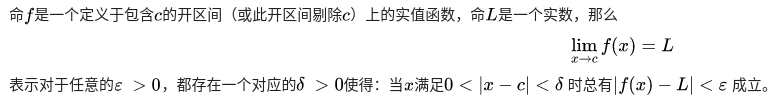
\includegraphics[width=15cm]{pictures_bitmap/wiki_limite.png}
\end{center}
Même pas besoin de connaitre la langue pour comprendre qu'il s'agit bien d'une limite épointée.
 
Contrairement à ce que certains laissent entendre, adopter la limite épointée n'est pas céder à la tradition anlgo-saxonne. C'est juste ce qui se fait partout.

On pourrait penser que ceci n'est pas un élément très lourd au dossier parce qu'il y a moyen d'être très bien tout en étant une spécificité française. C'est le cas par exemple de la notation \( \mathopen] a , b \mathclose[\) pour l'intervalle ouvert.

%///////////////////////////////////////////////////////////////////////////////////////////////////////////////////////////
\subsubsection{La limite épointée est plus riche}
%///////////////////////////////////////////////////////////////////////////////////////////////////////////////////////////

La classe des fonction admettant une limite pointée est plus grande que celle admettant une limite épointée (lemme \ref{LEMooWAZLooDPvemu}). L'utilisation de la limite épointée permet de décrire quelque cas supplémentaires par rapport à ce que l'on peut faire seulement avec la limite pointée.

Pour être plus précis, comme je le disait précédemment, en \ref{NORMooSLAJooLfDreV}, aucune des deux notions n'est satisfaisante seule :
\begin{itemize}
    \item mettez de la limite pointée dans les hypothèses, vous aurez un théorème moins général;
    \item mettez de la limite pointée dans la thèse, vous aurez un résultat plus fort.
\end{itemize}

Le vrai intérêt de la limite épointée est que \emph{en combinaison avec la notion de continuité} permet d'être plus général et plus précis que ce qu'on peut obtenir avec la limite pointée. Dit autrement, le couple (limite épointée, continuité) est plus fort que le couple (limite pointée, continuité).

D'un certain point de vue, oui, la limite pointée est plus simple, mais elle est plus simple parce qu'elle donne moins d'informations.

%///////////////////////////////////////////////////////////////////////////////////////////////////////////////////////////
\subsubsection{Retour sur le théorème de composition}
%///////////////////////////////////////////////////////////////////////////////////////////////////////////////////////////

Le \emph{vrai} théorème de composition est le théorème \ref{THOooHXGIooBclAHA}. Lui, il passe en revue tous les cas possibles et donne le plus de conclusions possibles dans chaque cas.

Ce théorème s'exprime de façon à peu près convenable à l'aide de limites et de continuité. J'attends de voir le même avec une limite pointée et la continuité.

Je suis très ouvert à la discussion si c'est pour avoir quelque chose de plus simple produisant les mêmes résultats. Je ne suis par contre pas très ouvert pour avoir quelque chose de plus simple, mais donnant moins de résultats. C'est toujours facile d'avoir des résultats plus courts, plus simples et plus intuitifs quand on se contente de moins.

%///////////////////////////////////////////////////////////////////////////////////////////////////////////////////////////
\subsubsection{La question est pédagogique}
%///////////////////////////////////////////////////////////////////////////////////////////////////////////////////////////

Tant qu'on ne m'a pas montré comment on exprime le théorème de composition \ref{THOooHXGIooBclAHA} avec des limites pointées, je resterai sur cette idée : la limite pointée est plus simple, mais elle dit moins.

Cela n'est cependant pas spécialement bloquant. Après tout, ça dépend de ce qu'on veut. D'un point de vue pédagogique, la limite pointée introduit autant de \( \epsilon\) et de \( \delta\) qu'on le veut, et permet d'introduire tous les concepts utiles en analyse.

La question est de savoir à quel point on est prêt à se compliquer la vie pour avoir des théorèmes un micro-cheveu plus complets. Le choix du Frido est de recevoir la difficulté avec résignation et de l'endurer avec courage, pour le plaisir d'avoir des théorèmes qui donnent un peu plus d'information\footnote{C'est une de mes citation préférées. Vu que nous sommes entre adultes je vous donne la référence : \cite{BIBooTOVWooSDsNrc}. Si vous n'avez pas 18 ans, on peut vraiment se demander si le Frido sont vraiment des lectures de votre âge.}.


%///////////////////////////////////////////////////////////////////////////////////////////////////////////////////////////
\subsubsection{En fait ça ne change presque rien}
%///////////////////////////////////////////////////////////////////////////////////////////////////////////////////////////

Certains s'imaginent qu'utiliser la limite pointée demande d'ajuster beaucoup de résultats un peu partout\cite{BIBooTOVWooSDsNrc}. Le Frido contient à ma connaissance seulement deux théorèmes dont l'énoncé contient une subtilité due au choix épointé. Le fameux théorème de composition \ref{THOooNPBQooEMOYpd}, et le lemme \ref{LEMooYLIHooFBQyzC}.

Le fait est que l'on ne calcule presque jamais de limites en une valeur où la fonction existe. Si on calcule une limite, c'est précisément parce qu'on regarde un point où la fonction n'existe pas.

Exemples:
\begin{itemize}
    \item Quand on calcule une dérivée, on calcule
        \begin{equation}
            \lim_{\epsilon\to 0}\frac{ f(a+\epsilon)-f(a) }{ \epsilon }.
        \end{equation}
        Cette fonction de \( \epsilon\) n'existe pas lorsque \( \epsilon=0\). Donc les limites pointées et épointées sont identiques.
    \item
        De même, l'étude du sinus cardinal \( f(x)=\sin(x)/x\) (lemme \ref{LEMooMJFBooAjtNjV}) est une fonction dont ça ne viendrait à l'idée de personne de calculer la limite pour \( x\to 4\). Et ça tombe bien : la seule limite que ça donne envie de calculer est
        \begin{equation}
            \lim_{x\to 0} \frac{ \sin(x) }{ x }.
        \end{equation}
        Et encore une fois, la fonction dans le limite n'existe pas au point limite.
    \item
        Toutes les conditions d'intégrabilité demandent des limites à l'infini. Là encore, ce sont des limites vers des points où la fonction n'existe pas. Franchement, qui va vouloir définir
        \begin{equation}
            \begin{aligned}
                f\colon \mathopen[ 0 , \infty \mathclose]&\to \eR \\
                x&\mapsto \begin{cases}
                    x^2    &   \text{si } x\neq \infty\\
                    0    &    \text{si } x=\infty
                \end{cases}
            \end{aligned}
        \end{equation}
        sans rigoler ?  Ok. Pour cette fonction, il y a une différence entre la limite pointée et épointée. Mais franchement, c'est bien la limite épointée qui donne le résultat «intuitif».
\end{itemize}


%///////////////////////////////////////////////////////////////////////////////////////////////////////////////////////////
\subsubsection{Et les filtres ?}
%///////////////////////////////////////////////////////////////////////////////////////////////////////////////////////////

Si vous ne savez pas ce qu'est un filtre, vous pouvez sauter ces paragraphes. Sinon, vous pouvez vous dire que le débat «limite pointée» contre «limite épointée» n'a aucun sens parce que de toutes façons, la bonne façon de définir une limite passe par des filtres.

Alors le mieux est de se demander comment on construit, à partir de la notion de filtre, le nombre \( \lim_{x\to a} f(a)\) ?

Pas de bol, ça dépend du filtre choisi. Le premier filtre auquel on pense pour trouver une définition raisonnable de la limite de \( f(x)\) quand \( x\to a\) est le filtre des voisinages de \( a\). La notion de limite associée est la limite pointée. En ce sens la limite pointée est plus naturelle\cite{BIBooWYHRooVGYMKV,BIBooHHPXooWbCAXQ} que la limite épointée. Cependant «naturel» signifie souvent «le premier qui nous tombe sous la main», ce qui ne signifie pas spécialement «le plus intéressant à utiliser».

La notion de limite épointée est la limite associée au filtre des voisinages épointés. Ce n'est, certes, pas le premier filtre qui nous tombe sous la main, mais il est, au moins dans le cadre de l'étude des fonctions sur \( \eR^n\), le plus efficace; celui qui donne le plus de nouvelles informations par rapport à la continuité.


%///////////////////////////////////////////////////////////////////////////////////////////////////////////////////////////
\subsubsection{En très résumé}
%///////////////////////////////////////////////////////////////////////////////////////////////////////////////////////////

Si vous ne voulez pas lire toute ma prose, voici mes arguments en très court.
\begin{enumerate}
    \item
        La limite épointée est celle utilisée partout sauf en France.
    \item
        La limite épointée est un peu plus compliquée que la limite pointée, mais elle permet de prouver plus de choses. En témoigne le théorème «complèt» de composition \ref{THOooHXGIooBclAHA} que je doute être facile à exprimer à l'aide des limites pointées et de la continuité\footnote{Il y a bien entendu moyen. Voir par exemple \cite{BIBooDAGXooRltbgK}. Sans ironie, je trouve ce théorème fascinant.}.
\end{enumerate}


%///////////////////////////////////////////////////////////////////////////////////////////////////////////////////////////
\subsubsection{Que devez-vous faire ?}
%///////////////////////////////////////////////////////////////////////////////////////////////////////////////////////////

\begin{description}
    \item[Enseignement en France] La notion de limite pointée est celle nommée «limite» dans les programmes, et ce que nous nommons ici «limite» est nommé «limite épointée». Peut-être pour induire en erreur tout le reste de la planète ?
    \item[Recherche] Si vous faites de la recherche où que ce soit y compris en France, la seule définition de limite est la limite dite «épointée», celle qui sera toujours utilisée dans le Frido.
    \item[Doctorat] Vous commencez un doctorat en math, et vous avez vu la limite pointée comme seule définition de limite durant vos études ? Oubliez-la. Ou alors attendez-vous à vous à de sérieux quiproquos lorsque vous discuterez de mathématique avec des étrangers. 

        Disons clairement que si vous utilisez la limite pointée devant des non Français, ils se diront juste que vous devriez relire vos cours de base. Et si vous leur expliquez, il y a de bonnes chance qu'ils ne vous croient pas.
\end{description}


%+++++++++++++++++++++++++++++++++++++++++++++++++++++++++++++++++++++++++++++++++++++++++++++++++++++++++++++++++++++++++++
\section{Continuité}
%+++++++++++++++++++++++++++++++++++++++++++++++++++++++++++++++++++++++++++++++++++++++++++++++++++++++++++++++++++++++++++

La définition de fonction continue est la définition~\ref{DefOLNtrxB}. Dans le cas d'une fonction \( f\colon \eR\to \eR\), elle devient ceci.
\begin{proposition}      \label{PROPooVNGEooPwbxXP}
    Soient \( A\subset \eR\) et \( a\in A\). La fonction \( f\colon A\to \eR\) est \defe{continue en $a$}{continue sur \( \eR\)} si et seulement si pour tout \( \epsilon>0\), il existe un \( \delta>0\) tel que si \( x\in B(a,\delta)\cap A\) alors \( | f(x)-f(a) |\leq \epsilon\).
\end{proposition}

Nous allons maintenant étudier quelques conséquences de la continuité sur \( \eR\).

\begin{enumerate}
\item D'abord on voit que la continuité n'a été définie qu'en un point. On peut dire que la fonction $f$ est continue \emph{en tel point donné}, mais nous n'avons pas dit ce qu'est une fonction continue \emph{dans son ensemble}.

\item
    Le théorème \ref{ThoESCaraB} nous précise que si $I$ est un intervalle de $\eR$, la fonction $f$ est continue sur $I$ si et seulement si elle est continue en chaque point de $I$.

\item Comme la définition de $f$ continue en $a$ fait intervenir $f(x)$ pour tous les $x$ pas trop loin de $a$, il faut au moins déjà que $f$ soit définie sur ces $x$. En d'autres termes, dire que $f$ est continue en $a$ demande que $f$ existe sur un intervalle autour de $a$.

Ceci couplé à la définition précédente laisse penser qu'il est surtout intéressant d'étudier les fonctions qui sont continues sur un intervalle.

\item L'intuition comme quoi une fonction continue doit pouvoir être tracée sans lever la main correspond aux fonctions continues sur des intervalles. Au moins sur l'intervalle où elle est continue, elle est traçable en un morceau.
\end{enumerate}

\begin{example}
    Il est très possible d'être continue en un seul point. Par exemple la fonction
    \begin{equation}
        f(x)=x(1-\mtu_{\eQ}(x))
    \end{equation}
    où \( \mtu_{\eQ}\) est la fonction indicatrice de \( \eQ\) dans \( \eR\).
\end{example}

\begin{proposition}     \label{PROPooUBUAooNIxjfg}
    Si \( f\colon \eR\to \eR\) est continue au point \( a\in \eR\) et si \( f(a)\neq 0\), alors il existe un voisinage de \( a\) sur lequel \( f\) ne s'annule pas.
\end{proposition}

\begin{proof}
    Si \( f \) s'annulait sur tout voisinage de \( a\) (mais pas ne \( a\) lui-même), nous aurions, pour tout \( n\) un réel
    \begin{equation}
        x_n\in B\big( a,\frac{1}{ n } \big)\setminus\{ a \}
    \end{equation}
    tel que \( f(x_n)=0\). Cela donnerait une suite \( x_n\to a\) avec \( f(x_n)\to 0\), ce qui contredit la continuité de \( f\) en \( a\) en vertu de la proposition \ref{PropFnContParSuite}\ref{ItemWJHIooMdugfu} sur la continuité séquentielle en un point.
\end{proof}

Notons que ce résultat se généralise beaucoup : si \( f\) est continue et pas égale à \( r\) en \( a\), alors elle continue à n'être pas égale à \( r\) dans un voisinage de \( a\).

%--------------------------------------------------------------------------------------------------------------------------- 
\subsection{Opération sur la continuité}
%---------------------------------------------------------------------------------------------------------------------------

Nous allons démontrer maintenant une série de petits résultats qui permettent de simplifier la démonstration de la continuité de fonctions.
\begin{theorem}
Si la fonction $f$ est continue au point $a$, alors la fonction $\lambda f$ est également continue en $a$.
\end{theorem}

\begin{proof}
Soit $\epsilon>0$. Nous avons besoin d'un $\delta>0$ tel que pour chaque $x$ à moins de $\delta$ de $a$, la fonction $\lambda f$ soit à moins de $\epsilon$ de $(\lambda f)(a)=\lambda f(a)$. Étant donné que la fonction $f$ est continue en $a$, on sait déjà qu'il existe un $\delta_1$ (nous notons $\delta_1$ afin de ne pas confondre ce nombre dont on est sûr de l'existence avec le $\delta$ que nous sommes en train de chercher) tel que
\[
  (| x-a |\leq \delta_1)\Rightarrow | f(x)-f(a) |\leq \epsilon_1.
\]
Hélas, ce $\delta_1$ n'est pas celui qu'il faut faut parce que nous travaillons avec $\lambda f$ au lieu de $f$, ce qui fait qu'au lieu d'avoir $| f(x)-f(a) |$, nous avons $| \lambda f(x)-\lambda f(a) |=| \lambda |\cdot | f(x)-f(a) |$.  Ce que $\delta_1$ fait avec $(\lambda f)$, c'est
\[
  (| x-a |\leq\delta_1)\Rightarrow  | (\lambda f)(x)- (\lambda f)(a)|\leq | \lambda |\epsilon_1.
\]
Ce que nous apprend la continuité de $f$, c'est que pour chaque choix de $\epsilon_1$, on a un $\delta_1$ qui fait cette implication. Comme cela est vrai pour chaque choix de $\epsilon_1$, essayons avec $\epsilon_1=\epsilon/| \lambda |$ pour voir ce que ça donne. Nous avons donc un $\delta_1$ qui fait
\[
  (| x-a |\leq\delta_1)\Rightarrow  | (\lambda f)(x)- (\lambda f)(a)|\leq | \lambda |\epsilon_1=\epsilon.
\]
Ce $\delta_1$ est celui qu'on cherchait.
\end{proof}

\begin{theorem}
Si $f$ et $g$ sont deux fonctions continues en $a$, alors la fonction $f+g$ est également continue en $a$.
\end{theorem}

\begin{proof}
La continuité des fonctions $f$ et $g$ au point $a$ fait en sorte que pour tout choix de $\epsilon_1$ et $\epsilon_2$, il existe $\delta_1$ et $\delta_2$ tels que
\[
  (| x-a |\leq \delta_1)\Rightarrow | f(x)-f(a) |\leq \epsilon_1.
\]
et
\[
  (| x-a |\leq \delta_2)\Rightarrow | g(x)-g(a) |\leq \epsilon_2.
\]
La quantité que nous souhaitons analyser est $| f(x)+g(x)-f(a)-g(a) |$. Tout le jeu de la démonstration de la continuité est de triturer cette expression pour en tirer quelque chose en termes de $\epsilon_1$ et $\epsilon_2$. Si nous supposons avoir pris $| x-a |$ plus petit en même temps que $\delta_1$ et que $\delta_2$, nous avons
\[
| f(x)+g(x)-f(a)-g(a) |\leq| f(x)-g(x) |+| g(x)-g(a) |\leq\epsilon_1+\epsilon_2
\]
en utilisant la formule générale $| a+b |\leq | a |+| b |$. Maintenant si on choisit $\epsilon_1$ et $\epsilon_2$ tels que $\epsilon_1+\epsilon_2<\epsilon$, et les $\delta_1$, $\delta_2$ correspondants, on a
\[
| f(x)+g(x)-f(a)-g(a) |\leq\epsilon,
\]
pourvu que $| x-a |$ soit plus petit que $\delta_1$ et $\delta_2$. Le bon $\delta$ à prendre est donc le minimum de $\delta_1$ et $\delta_2$ qui eux-mêmes sont donnés par un choix de $\epsilon_1$ et $\epsilon_2$ tels que $\epsilon_1+\epsilon_2\leq\epsilon$.
\end{proof}

Pour résumer ces deux théorèmes, on dit que si $f$ et $g$ sont continues en $a$, alors la fonction $\alpha f+\beta g$ est également continue en $a$ pour tout $\alpha$, $\beta\in\eR$.

\begin{proposition}     \label{PROPooVNKVooJvxarf}
    Soient des parties \( \Omega_f\) et \( \Omega_g\) dans \( \eR\). Soient \( f\colon \Omega_f\to \eR\) ainsi que \( g\colon \Omega_g\to \eR\) telles que
    \begin{enumerate}
        \item
            \( g\) est continue en \( a\) et vaut \( g(a)=\ell\).
        \item
            \( f\) est continue en \( \ell\) et vaut \( f(\ell)=b\).
        \item
            \( g(\Omega_g)\subset \Omega_f\).
    \end{enumerate}
    Alors \( f\circ g\) est continue en \( a\).
\end{proposition}

\begin{proof}
    Soit \( \epsilon>0\). La continuité de \( f\) dit que il existe \( \eta>0\) tel que
    \begin{equation}
        y\in B(\ell,\eta)\cap\Omega_f\Rightarrow\,| f(y)-f(\ell) |<\epsilon.
    \end{equation}
    La continuité de \( g\) donne \( \delta>0\) tel que
    \begin{equation}
        x\in B(a,\delta)\cap\Omega_g\Rightarrow\,| g(x)-g(a) |<\eta.
    \end{equation}

    Si \( x\in B(a,\delta)\cap\Omega_g\), alors \( g(x)\in B(\ell,\eta)\cap\Omega_f\). Donc
    \begin{equation}
        | (f\circ g)(x)-f(\ell) |<\epsilon.
    \end{equation}
    Mais \( f(\ell)=(f\circ g)(a)\). Tout cela est la continuité de \( f\circ g\) en \( a\).
\end{proof}


Parmi les propriétés immédiates de la continuité d'une fonction, nous avons ceci qui est souvent bien utile.

\begin{corollary}   \label{CorNNPYooMbaYZg}
Si la fonction $f$ est continue en $a$ et si $f(a)>0$, alors $f$ est positive sur un intervalle autour de $a$.
\end{corollary}

\begin{proof}
Prenons $\epsilon<f(a)$ et voyons\footnote{ici, nous insistons sur le fait que nous prenons $\epsilon$ \emph{strictement} plus petit que $f(a)$.} ce que la continuité de $f$ en $a$ nous offre : il existe un $\delta$ tel que
\[
  (| x-a |\leq \delta)\Rightarrow | f(x)-f(a) |\leq\epsilon < f(a).
\]
Nous en retenons que sur un intervalle (de largeur $\delta$), nous avons $| f(x)-f(a) |\leq f(a)$. Par hypothèse, $f(a)>0$, donc si $f(x)<0$, alors la différence $f(x)-f(a)$ donne un nombre encore plus négatif que $-f(a)$, c'est-à-dire que $| f(x)-f(a) |>f(a)$, ce qui est contraire à ce que nous venons de démontrer. D'où la conclusion que $f(x)>0$.
\end{proof}

\subsection{La fonction la moins continue du monde}
%--------------------------------------------------

Parmi les exemples un peu sales de fonctions non continues, il y a celle-ci :
\[
  \chi_{\eQ}(x)=
\begin{cases}
    1 \text{ si }x\in\eQ\\
    0 \text{ sinon.}
\end{cases}
\]
Par exemple, $\chi_{\eQ}(0)=1$, et\footnote{Pour prouver que $\sqrt{2}$ n'est pas rationnel, c'est pas trop compliqué, mais pour prouver que $\pi$ ne l'est pas non plus, il faudra encore manger de la soupe.} $\chi_{\eQ}(\pi)=\chi_{\eQ}(\sqrt{2})=0$. Malgré que $\chi_{\eQ}(0)=1$, il n'existe \emph{aucun} voisinage de $1$ sur lequel la fonction reste proche de $1$, parce que tout voisinage va contenir au moins un irrationnel. À chaque millimètre, cette fonction fait une infinité de bonds !

Cette fonction n'est donc continue nulle part.

À partir de là, nous pouvons construire la fonction suivante qui n'est continue qu'en un point :
\[
  f(x)=x\chi_{\eQ}(x)=
\begin{cases}
x\text{ si }x\in\eQ\\
0\text{ sinon.}
\end{cases}
\]
Cette fonction est continue en zéro. En effet, prenons $\delta>0$; il nous faut un $\epsilon$ tel que $| x |\leq\epsilon$ implique $f(x)\leq \delta$ parce que $f(0)=0$. Bon ben prendre simplement $\epsilon=\delta$ nous contente. Cette fonction est donc très facilement continue en zéro.

Et pourtant, dès que l'on s'écarte un tant soit peu de zéro, elle fait des bons une infinité de fois par millionième de millimètre ! Cette fonction est donc la plus discontinue du monde en tous les points saut un (zéro) où elle est une fonction continue !

\subsection{Approche topologique}
%--------------------------------

Nous avons vu que sur tout ensemble métrique, nous pouvons définir ce qu'est un ouvert : c'est un ensemble qui contient une boule ouverte autour de chacun de ses points. Quand on est dans un ensemble ouvert, on peut toujours un peu se déplacer sans sortir de l'ensemble.

Le théorème suivant est une très importante caractérisation des fonctions continues (de $\eR$ dans $\eR$) en termes de topologie, c'est-à-dire en termes d'ouverts.

\begin{theorem}     \label{ThoContInvOuvert}
Si $I$ est un intervalle ouvert contenu dans $\dom f$, alors $f$ est continue sur $I$ si et seulement si pour tout ouvert $\mO$ dans $\eR$, l'image inverse $f|_I^{^{-1}}(\mO)$ est ouvert.
\end{theorem}

Par abus de langage, nous exprimons souvent cette condition par « une fonction est continue si et seulement si l'image inverse de tout ouvert est un ouvert ».

\begin{proof}

Dans un premier temps, nous allons transformer le critère de continuité en termes de boules ouvertes, et ensuite, nous passerons à la démonstration proprement dite. Le critère de continuité de $f$ au point $x$ dit que
\begin{equation}        \label{EqDEfCOntAn}
  \forall \delta>0,\exists\,\epsilon>0\text{ tel que }\big( | x-a |< \epsilon \big)\Rightarrow| f(x)-f(a) |<\delta.
\end{equation}
Cette condition peut être exprimée sous la forme suivante :
\[
  \forall \delta>0,\exists\epsilon\text{ tel que } a\in B(x,\epsilon)\Rightarrow f(a)\in B\big( f(x),\delta \big),
\]
ou encore
\begin{equation}        \label{EqRedefContBoules}
  \forall \delta>0,\exists\epsilon\text{ tel que } f\big( B(x,\epsilon) \big)\subset B\big( f(x),\delta \big).
\end{equation}
Jusque ici, nous n'avons fait que du jeu de notations. Nous avons exprimé en termes de topologie des inégalités analytiques. La condition \eqref{EqRedefContBoules} est le plus souvent utilisée comme définition de la continuité d'une fonction en \( x\), lorsque le contexte ne demande pas de définitions plus générales. Si tel est le choix, il faut pouvoir retrouver \eqref{EqDEfCOntAn} à partir de \eqref{EqRedefContBoules}.

Passons maintenant à la démonstration proprement dite du théorème.

D'abord, supposons que $f$ est continue sur $I$, et prenons $\mO$, un ouvert quelconque. Le but est de prouver que $f|_I^{-1}(\mO)$ est ouvert. Pour cela, nous prenons un point $x_0\in f|_I^{-1}(\mO)$ et nous allons trouver un ouvert autour ce point contenu dans $f|_I^{-1}(\mO)$. Nous écrivons $y_0=f(x_0)$. évidemment, $y_0\in\mO$, donc on a une boule autour de $y_0$ qui est contenue dans $\mO$, soit donc $\delta>0$ tel que
\[
  B(y_0,\delta)\subset\mO.
\]
Par hypothèse, $f$ est continue en $x_0$, et nous pouvons donc y appliquer le critère \eqref{EqRedefContBoules}. Il existe donc $\epsilon>0$ tel que
\[
  f\big( B(x_0,\epsilon) \big)\subset B\big( f(x_0),\delta \big)\subset\mO.
\]
Cela prouve que $B(x_0,\epsilon)\subset f|_I^{-1}(\mO)$.

Dans l'autre sens, maintenant. Nous prenons $x_0\in I$ et nous voulons prouver que $f$ est continue en $x_0$, c'est-à-dire que pour tout $\delta$ nous cherchons un $\epsilon$ tel que $f\big( B(x_0,\epsilon) \big)\subset B\big( f(x_0),\delta \big)$. Oui, mais $B\big( f(x_0),\delta \big)$ est ouverte, donc par hypothèse, $f|_I^{-1}\Big( B\big( f(x_0),\delta \big) \Big)$ est ouvert, inclus dans $I$ et contient $x_0$. Donc il existe un $\epsilon$ tel que
\[
  B(x_0,\epsilon)\subset f|_I^{-1}\Big( B\big( f(x_0),\delta \big) \Big),
\]
et donc tel que
\[
  f\big( B(x_0,\epsilon) \big)\subset B\big( f(x_0),\delta \big),
\]
ce qu'il fallait prouver.
\end{proof}

\begin{lemma}   \label{LemConncontconn}
L'image d'un ensemble connexe par une fonction continue est connexe.
\end{lemma}

\begin{proof}
Nous allons encore faire la contraposée. Soit $A$ une partie de $\eR$ telle que $f(A)$ ne soit pas connexe. Nous allons prouver que $A$ elle-même n'est pas connexe. Dire que $f(A)$ n'est pas connexe, c'est dire qu'il existe $\mO_1$ et $\mO_2$, deux ouverts disjoints qui recouvrent $f(A)$. Je prétends que $f^{-1}(\mO_1)$ et $f^{-1}(\mO_2)$ sont ouverts, disjoints et qu'ils recouvrent $A$.
\begin{itemize}
\item Ces deux ensembles sont ouverts parce qu'ils sont images inverses d'ouverts par une fonction continue (théorème~\ref{ThoContInvOuvert}).
\item Si $x\in f^{-1}(\mO_1)\cap f^{-1}(\mO_2)$, alors $f(x)\in \mO_1\cap\mO_2$, ce qui contredirait le fait que $\mO_1$ et $\mO_2$ sont disjoints. Il n'y a donc pas d'éléments dans l'intersection de $f^{-1}(\mO_1)$ et de $f^{-1}(\mO_2)$.
\item Si $f^{-1}(\mO_1)$ et $f^{-1}(\mO_2)$ ne recouvrent pas $A$, il existe un $x$ dans $A$ qui n'est dans aucun des deux. Dans ce cas, $f(x)$ est dans $f(A)$, mais n'est ni dans $\mO_1$, ni dans $\mO_2$, ce qui contredirait le fait que ces deux derniers recouvrent $f(A)$.
\end{itemize}
Nous déduisons que $A$ n'est pas connexe. Et donc le lemme.
\end{proof}

\begin{theorem}[Théorème des valeurs intermédiaires]        \label{ThoValInter}
    Soit $f$, une fonction continue sur $[a,b]$, et supposons que $f(a)<f(b)$. Alors pour tout $y$ tel que $f(a)\leq y\leq f(b)$, il existe un \( x\in\mathopen[ a , b \mathclose]\) tel que $f(x)=y$.
\end{theorem}
\index{connexité!théorème des valeurs intermédiaires}
\index{théorème!valeurs intermédiaires}

\begin{proof}
Nous savons que $[a,b]$ est connexe parce que c'est un intervalle (proposition~\ref{PropInterssiConn}). Donc $f\big( [a,b] \big)$ est connexe (lemme~\ref{LemConncontconn}) et donc est un intervalle (à nouveau la proposition~\ref{PropInterssiConn}). Étant donné que $f\big( [a,b] \big)$ est un intervalle, il contient toutes les valeurs intermédiaires entre n'importe quels deux de ses éléments. En particulier toutes les valeurs intermédiaires entre $f(a)$ et $f(b)$.
\end{proof}

\begin{corollary}       \label{CorImInterInter}
L'image d'un intervalle par une fonction continue est un intervalle.
\end{corollary}

\begin{proof}
Soient \( I\) un intervalle, \( \alpha<\beta\in f(I)\) et \( \gamma\in\mathopen] \alpha , \beta \mathclose[\). Nous considérons \(a,b\in I\) tels que \( \alpha=f(a)\) et \( \beta=f(b)\). Par le théorème des valeurs intermédiaires \ref{ThoValInter}, il existe \( t\in\mathopen] a , b \mathclose[\) tel que \( f(t)=\gamma\). Par conséquent \( \gamma\in f(I)\).
\end{proof}

\begin{corollaryDef}[Existence de la racine carrée]     \label{DEFooGQTYooORuvQb}
    Si \( x\geq 0\) alors il existe un unique \( y\geq 0\) tel que \( y^2=x\). Ce nombre est noté \( \sqrt{x}\) et est nommé \defe{racine carrée}{racine carrée} de \( x\).
\end{corollaryDef}

\begin{proof}
    La fonction \( f\colon t\mapsto t^2\) est continue et strictement croissante. Nous avons \( f(0)=0\) et\footnote{Faites deux cas suivant \( x\geq 1\) ou non si vous le voulez, moi je prends \( x+1\).} \( f(x+1)>x\). Donc le théorème des valeurs intermédiaires~\ref{ThoValInter} nous assure qu'il existe un unique \( y\in\mathopen[ 0 , x+1 \mathclose]\) tel que \( f(y)=x\).
\end{proof}

\begin{lemma}       \label{LEMooSBOAooOOIotR}
    La fonction racine carrée est strictement croissante.
\end{lemma}

\begin{proof}
    Supposons que \( x<y\). Si \( \sqrt{ x }>\sqrt{ y }\), alors la croissance de la fonction carré donne \( x>y\) qui est contraire à l'hypothèse..
\end{proof}

%--------------------------------------------------------------------------------------------------------------------------- 
\subsection{Module sur les nombres complexes}
%---------------------------------------------------------------------------------------------------------------------------

\begin{lemmaDef}
    Si \( z\in \eC\), alors \( z\bar z\) est un réel positif.

    Nous définissons le \defe{module}{module d'un nombre complexe} sur \( \eC\) par\footnote{Définition de la racine carré : \ref{DEFooGQTYooORuvQb}.}
    \begin{equation}
        | z |=\sqrt{ z\bar z }.
    \end{equation}
\end{lemmaDef}

\begin{proof}
    Prouvons que \( z\bar z\) est un réel positif. En effet si \( z=a+bi\) alors
    \begin{equation}
        z\bar z=(a+bi)(a-bi)=a^2-abi+abi+b^2=a^2+b^2\geq 0.
    \end{equation}
\end{proof}

\begin{proposition}     \label{PROPooUMVGooIrhZZg}
Pour tout nombres complexes $z = a+bi$ et $z^\prime$, nous avons
   \begin{enumerate}
   \item $z \bar z = a^2 + b^2$;
   \item $\bar{\bar{z}} = z$;
   \item $\module z = \module {\bar z}$;
   \item        \label{ITEMooFXKYooUOXbwH}
       $\module{zz^\prime} = \module z \module{z^\prime}$;        
   \item    \label{ITEMooDVMDooFDmOur}
      \( | z_1+z_2 |\leq | z_1 |+| z_2 |\)
   \end{enumerate}
\end{proposition}


\begin{lemma}       \label{LEMooHTAWooQNrXSL}
    Nous avons \( | \real(z) |\leq | z |\) et nous avons l'égalité si et seulement si \( z\in \eR\).
\end{lemma}

\begin{proof}
    En plusieurs points.
    \begin{subproof}
    \item[L'inégalité]
        Par croissance de la fonction racine carré nous avons, en posant \( z=a+bi\) :
        \begin{equation}        \label{EQooBFANooKcSsWi}
            | \real(z) |=| a |=\sqrt{ | a |^2 }\leq \sqrt{ | a |^2+| b |^2 }=| z |.
        \end{equation}
    \item[Égalité dans un sens]
        Si \( | \real(z) |=| z |\), alors toutes les inégalités dans \eqref{EQooBFANooKcSsWi} sont des égalités. En particulier
        \begin{equation}
            \sqrt{ | a |^2 }=\sqrt{ | a |^2+| b |^2 }.
        \end{equation}
        Par stricte croissance de la fonction racine carré, nous déduisons que \( | b |^2=0\) et donc que \( b=0\).
    \item[Égalité dans l'autre sens]
        Si \( z\in \eR\), alors \( \real(z)=z\), et nous avons l'égalité.
    \end{subproof}
\end{proof}

\begin{lemma}       \label{LEMooHWLXooSkUrGg}
    Soient \( a,b\in \eC\). Nous avons \( | a+b |=| a |+| b |\) si et seulement si \( a\bar b=0\).
\end{lemma}

\begin{proof}
    Nous avons toujours l'égalité
    \begin{equation}
        | a+b |=\sqrt{ | a |^2+| b |^2+2\real(a\bar b) }.
    \end{equation}

    Dans un premier sens nous supposons \( | a+b |=| a |+| b |\). Donc 
    \begin{equation}
        \sqrt{ | a |^2+| b |^2+2\real(a\bar b) }=\sqrt{ | a |^2+| b |^2+2| a | |b | },
    \end{equation}
    et donc que \( \real(a\bar b)=| a | |b |\). Vu que \( | a\bar b |=| a | |b |\) (proposition \ref{PROPooUMVGooIrhZZg}\ref{ITEMooFXKYooUOXbwH}), nous avons
    \begin{equation}
        \real(a\bar b)=| a\bar b |.
    \end{equation}
    Nous sommes dans le cas d'égalité du lemme \ref{LEMooHTAWooQNrXSL}. Donc \( a\bar b\in \eR\). Et il est manifestement positif parce que égal à \( | a | |b |\).

     Dans l'autre sens, nous supposons que \( a\bar b=0\). En particulier \( a\bar b\in \eR\) et \( \real(a\bar b)=| a | |b |\). Nous avons alors
    \begin{equation}
        | a+b |=\sqrt{ | a |^2+| b |^2+2\real(a\bar b) }=| a |+| b |.
    \end{equation}
\end{proof}

\begin{lemma}       \label{LEMooRJICooYrcAFv}
    À propos du module.
    \begin{enumerate}
        \item       \label{ITEMooCTHXooHqzuvb}
            Si \( x,y\in \eC\) nous avons
    \begin{equation}
        | x+y |\leq | x |+| y |.
    \end{equation}
        \item
            Il y a égalité si et seulement si \( x\bar y\geq 0\).
    \end{enumerate}
\end{lemma}

\begin{proof}
    En plusieurs points.
    \begin{subproof}
    \item[L'inégalité]
            Nous considérons deux nombres complexes \( x\) et \( y\). Nous avons
            \begin{equation}
                | x+y |=\sqrt{ | x |^2+| y |^2+x\bar y+\bar xy }.
            \end{equation}
            Maintenant, \( x\bar y+y\bar x=2\real(xy)\) et \( \real(z)\leq | z |\) et la racine carré est croissante\footnote{Lemme \ref{LEMooSBOAooOOIotR}.}. Donc
            \begin{equation}
                | x+y |=\sqrt{ | x |^2+| y |^2+x\bar y+\bar xy }\leq \sqrt{ | x |^2+| y |^2+2| x\bar y | }=\sqrt{ | x |^2+| y |^2+2| x | |y | }=| x |+| y |.
            \end{equation}
        \item[Le cas d'égalité]
            C'est le lemme \ref{LEMooHWLXooSkUrGg}.
    \end{subproof}
\end{proof}

\begin{lemma}       \label{LEMooXJBJooFDmhnV}
    Si deux nombres complexes \( a,b\in \eC\) vérifient \( a\bar b\in \eR\), alors on est dans un des deux cas suivants :
    \begin{itemize}
        \item \( b=0\)
        \item il existe \( \lambda\in \eR\) tel que \( a=\lambda b\).
    \end{itemize}
    De façon équivalente, il existe \( \alpha,\beta\in \eR\) non tous deux nuls tels que \( \alpha a+\beta b=0\).
\end{lemma}

\begin{proof}
    Nous écrivons \( a=a_1+ia_2\) et \( b=b_1+ib_2\) avec \( a_i,b_i\in \eR\). Nous supposons \( b\neq 0\). Nous effectuons la multiplication \( a\bar b=(a+ib_2)(b_1-ib_2)\) et nous annulons la partie imaginaire :
    \begin{equation}
        a_2b_1-a_1b_2=0.
    \end{equation}
    Si \( b_1=0\) alors \( a_1b_2=0\) avec \( b_2\neq 0\), ce qui implique \( a_1=0\). Donc \( a=ia_2\), \( b=ib_2\). Résultat obtenu.

    Si \( b_1\neq 0\) alors 
    \begin{equation}
        a_2=\frac{ a_1b_2 }{ b_1 },
    \end{equation}
    et nous avons du coup
    \begin{equation}
        a=\frac{ a_1 }{ b_1 }b.
    \end{equation}
    Mission accomplie.

    Nous prouvons à présent la formulation équivalente. Si \( b=0\) il suffit de prendre \( \alpha=0\). Si \( a=\lambda b\) il faut prendre \( \alpha=\beta/\lambda\).

    Dans l'autre sens, si \( \alpha\neq 0\) alors \( a=-(\beta/\alpha)b\) et si \( \alpha=0\) alors \( \beta\neq 0\) et il reste \( b=0\).
\end{proof}

\begin{proposition}
    La paire \( (\eC, | . |)\) est un espace vectoriel normé\footnote{Définition d'une norme : \ref{DefNorme}.}.
\end{proposition}

\begin{proof}
    Nous devons prouver les différents points de la définition \ref{DefNorme}.
    \begin{enumerate}
        \item
            \( | z |\geq 0\) parce que la racine carré prend ses valeurs dans \( \eR^+\).
        \item
            Si \( | z |=0\), alors, en notant \( z=a+bi\) nous avons \( a^2+b^2=0\). La somme de deux positifs est nulle que quand les deux sont nuls. Donc \( a=b=0\).
        \item
            Si \( \lambda\geq 0\), alors \( (\lambda z)\overline{ \lambda z }=\lambda^2z\bar z\) et nous avons
            \begin{equation}
                | \lambda z |=\sqrt{ \lambda^2z\bar z }=| \lambda |\sqrt{ z\bar z }=| \lambda | |z |.
            \end{equation}
        \item
            L'inégalité \( | x+y |\leq | x |+| y |\) est le lemme \ref{LEMooRJICooYrcAFv}.
    \end{enumerate}
\end{proof}



\begin{proposition} \label{PROPooXLARooYSDCsF}
 Si \( z_1\) et \( z_2\) sont des nombres complexes, alors 
 \begin{equation}
     | z_1z_2 |=| z_1 | |z_2 |.
 \end{equation}
 Nous avons aussi, pour tout \( n\in \eN\),
 \begin{equation}       \label{EQooATTQooRpJeCo}
     | z^n |=| z |^n.
 \end{equation}
\end{proposition}

\begin{proof}
    D'abord \( (a+bi)(c+di)=ac-db+(ad+bc)i\), de telle sorte que
    \begin{equation}
        | (a+bi)(c+di) |^2=(ac-bd)^2+(ad+bc)^2.
    \end{equation}
    Mais en calculant d'autre part \( | a+bi |^2| c+di |^2\), nous tombons sur la même valeur.

    Une simple récurrence permet de conclure que \( | z^n |=| z |^n\).
\end{proof}
Voila. Vous êtes déjà content d'apprendre que l'on peut démontrer \( | z^n |=| z |^n\) sans faire appel à la forme trigonométrique des nombres complexes.


\begin{lemma}   \label{LEMooONLNooXLNbtB}
    Pour tout \( z\in \eC\) nous avons \( z\bar z=\bar z z=| z |^2\).
\end{lemma}



\subsection{Continuité de la racine carrée, invitation à la topologie induite}
%-----------------------------------------

Pourquoi nous intéresser particulièrement à cette fonction ? Parce qu'elle a une sale condition d'existence : son domaine de définition n'est pas ouvert. Or dans tous les théorèmes de continuité d'approche topologique que nous avons vus, nous avons donné des conditions \emph{pour tout ouvert}. Nous nous attendons donc a avoir des difficultés avec la continuité de $\sqrt{x}$ en zéro.

Prenons $I$, n'importe quel intervalle ouvert dans $\eR^+$, et voyons que la fonction\footnote{La racine carré est définie en \ref{DEFooGQTYooORuvQb}.}
\begin{equation}
\begin{aligned}
 f\colon \eR^+&\to \eR^+ \\
   x&\mapsto \sqrt{x}
\end{aligned}
\end{equation}
est continue sur $I$. Remarque déjà que si $I$ est un ouvert dans $\eR^+$, il ne peut pas contenir zéro. Avant de nous lancer dans notre propos, nous prouvons un lemme qui fera tout le travail\footnote{C'est toujours ingrat d'être un lemme : on fait tout le travail et c'est toujours le théorème qui est nommé.}.

\begin{lemma}
Soit $\mO$, un ouvert dans $\eR^+$. Alors $\mO^2=\{ x^2\tq x\in\mO \}$ est également ouvert .
\end{lemma}

\begin{proof}
Un élément de $\mO^2$ s'écrit sous la forme $x^2$ pour un certain $x\in\mO$. Le but est de trouver un ouvert autour de $x^2$ qui soit contenu dans $\mO^2$. Étant donné que $\mO$ est ouvert, on a une boule centrée en $x$ contenue dans $\mO$. Nous appelons $\delta$ le rayon de cette boule :
\[
  B(x,\delta)\subset\mO.
\]
Étant donné que cet ensemble est connexe, nous savons par le lemme~\ref{LemConncontconn} que $B(x,\delta)^2$ est également connexe (parce que la fonction $x\mapsto x^2$ est continue). Son plus grand élément est $(x+\delta)^2=x^2+\delta^2+2x\delta>x^2+\delta^2$, et son plus petit élément est $(x-\delta)^2=x^2+\delta^2-2x\delta$.

Ce qui serait pas mal, c'est que ces deux bornes entourent $x^2$; de cette façon elles définiraient un ouvert autour de $x^2$ qui soit dans $\mO^2$. Hélas, c'est pas gagné que $x^2+\delta^2-2x\delta$ soit plus petit que $x^2$.

Heureusement, en fait c'est vrai parce que d'une part, du fait que $\mO\subset\eR^+$, on a $x>0$, et d'autre part, pour que $\mO$ soit positif, il faut que $\delta<x$. Donc on a évidemment que $\delta<2x$, et donc que
\[
  x^2+\delta^2-2x\delta=x^2+\delta\underbrace{(\delta-2x)}_{<0}<x^2.
\]
Donc nous avons fini : l'ensemble
\[
  B(x,\delta)^2=]x^2+\delta^2-2x\delta,x^2+\delta^2+2x\delta[\subset\mO^2
\]
est un intervalle qui contient $x^2$, et donc qui contient une boule ouverte centrée en~$x^2$.

\end{proof}

Maintenant nous pouvons nous attaquer à la continuité de la racine carrée sur tout ouvert positif en utilisant le théorème~\ref{ThoContInvOuvert}. Soit $\mO$ n'importe quel ouvert de $\eR$, et prouvons que $f|_I^{-1}(\mO)$ est ouvert. Par définition,
\begin{equation}
  f|_I^{-1}(\mO)=\{ x\in I\tq \sqrt{x}\in\mO \}.
\end{equation}
Maintenant c'est un tout petit effort que de remarquer que $f|_I^{-1}(\mO)=\mO^2\cap I$. De là, on a gagné parce que $\mO^2$ et $I$ sont des ouverts. Or l'intersection de deux ouverts est ouvert.

Nous n'en avons pas fini avec la fonction $\sqrt{x}$. Nous avons la continuité de la racine carrée pour tous les réels strictement positifs. Il reste à pouvoir dire que la fonction est continue en zéro malgré qu'elle ne soit pas définie sur un ouvert autour de zéro.

Il est possible de dire que la racine carrée est continue en $0$, malgré qu'elle ne soit pas définie sur un ouvert autour de $0$\ldots en tout cas pas un ouvert au sens que tu as en tête. Nous allons rentabiliser un bon coup notre travail sur les espaces métriques.

Nous pouvons définir la notion de boule ouverte sur n'importe quel espace métrique $A$ en disant que
\[
  B(x,r)=\{ y\in A\tq d(x,y)<r \}.
\]
\begin{definition}      \label{DefContMetrique}
Soit $f\colon A\to B$, une application entre deux espaces métriques. Nous disons que $f$ est \defe{continue}{continue!sur espace métrique} au point $a\in A$ si $\forall \delta>0$, $\exists\epsilon>0$ tel que
\begin{equation}
  f\big( B(a,\epsilon) \big)\subset B\big( f(a),\delta \big).
\end{equation}
\end{definition}
Tu reconnais évidemment la condition \eqref{EqRedefContBoules}. Nous l'avons juste recopiée. Tu remarqueras cependant que cette définition généralise immensément la continuité que l'on avait travaillé à propos des fonctions de $\eR$ vers $\eR$. Maintenant tu peux prendre n'importe quel espace métrique et c'est bon.

Nous n'allons pas faire un tour complet des conséquences et exemples de cette définition. Au lieu de cela, nous allons juste montrer en quoi cette définition règle le problème de la continuité de la racine carrée en zéro.

La fonction que nous regardons est
\begin{equation}
\begin{aligned}
f \colon \eR^+&\to \eR^+ \\
   x&\mapsto \sqrt{x}.
\end{aligned}
\end{equation}
Mais cette fois, nous ne la voyons pas comme étant une fonction dont le domaine est une partie de $\eR$, mais comme fonction dont le domaine est $\eR^+$ vu comme un espace métrique en soi. Quelles sont les boules ouvertes dans $\eR^+$ autour de zéro ? Réponse : la boule ouverte de rayon $r$ autour de zéro dans $\eR^+$ est :
\[
  B(0,r)_{\eR^+}=\{ x\in\eR^+\tq d(x,0)<r \}=[0,r[.
\]
Cet intervalle est un ouvert. Aussi incroyable que cela puisse paraitre !

Testons la continuité de la racine carrée en zéro dans ce contexte. Il s'agit de prendre $A=\eR^+$, $B=\eR^+$ et $a=0$ dans la définition~\ref{DefContMetrique}. Nous avons que $B(\sqrt{0},\delta)=B(0,\delta)=[0,\delta[$ pour la topologie de $\eR^+$.

Il s'agit maintenant de trouver un $\epsilon$ tel que $f\big( B(0,\epsilon) \big)\subset [0,\delta[$. Par définition, nous avons que
\[
  f\big( B(0,\epsilon) \big)=[0,\sqrt{\epsilon}[,
\]
le problème revient dont à trouver $\epsilon$ tel que $\sqrt{\epsilon}\leq\delta$. Prendre $\epsilon<\delta^2$ fait l'affaire.

Donc voilà. Au sens de la topologie induite\footnote{Définition \ref{DefVLrgWDB}.}, de \( \eR\) vers $\eR^+$, nous pouvons dire que la fonction racine carrée est partout continue.

%--------------------------------------------------------------------------------------------------------------------------- 
\subsection{Second degré}
%---------------------------------------------------------------------------------------------------------------------------

Nous résolvons à présent le polynôme du second degré.
\begin{proposition}[\cite{BIBooYVBZooOrTJTr}]       \label{PROPooEZIKooKjJroH}
    Soit la fonction
    \begin{equation}
        \begin{aligned}
            f\colon \eR&\to \eR \\
            x&\mapsto ax^2+bx+c 
        \end{aligned}
    \end{equation}
    avec \( a\neq 0\). Nous notons \( \Delta=b^2-4ac\).

    \begin{enumerate}
        \item       \label{ITEMooMKUSooWwNTba}
            Nous avons la formule
            \begin{equation}        \label{EQooFKPOooAbIhCx}
                f(x)=a\big( x+\frac{ b }{ 2a } \big)^2+c-\frac{ b^2 }{ 4a }.
            \end{equation}
        \item       \label{ITEMooHQTBooZuaPAs}
            Si \( a>0\), alors \( f\) a un minimum global en \( x_m=-b/2a\).
        \item       \label{ITEMooQMXVooWsqiXz}
            Si \( a<0\), alors \( f\) a un maximum global en \( x_M=-b/2a\).
        \item       \label{ITEMooMAMHooNWZVQI}
            Si \( \Delta<0\) alors \( f\) ne possède pas de racines réelles.
        \item       \label{ITEMooKUUJooTsIHhI}
            Si \( \Delta=0\), alors \( f\) possède une unique racine \( x_0=-b/2a\).
        \item       \label{ITEMooQZGFooEGhMkX}
            Si \( \Delta>0\) alors \( f\) possède exactement deux racines distinctes données par
            \begin{equation}        \label{EQooGHDPooVkqINr}
                \begin{aligned}[]
                    x_1&=\frac{ -b+\sqrt{ \Delta } }{ 2a }&x_2&=\frac{ -b-\sqrt{ \Delta } }{ 2a }.
                \end{aligned}
            \end{equation}
    \end{enumerate}
\end{proposition}

\begin{proof}
    En plusieurs parties.
    \begin{subproof}
    \item[Pour \ref{ITEMooMKUSooWwNTba}]
        C'est un calcul immédiat.
    \item[Pour \ref{ITEMooHQTBooZuaPAs}]
        Nous partons de la formule du point \ref{ITEMooMKUSooWwNTba}. Vu que \( c-\frac{ b^2 }{ 4a }\) est constant, minimiser \( f\) revient à minimiser \( x\mapsto \big( x+\frac{ b }{ 2a } \big)^2\). Comme cette dernière fonction est toujours positive, elle a un minimum global là où elle est nulle, c'est à dire en \( x_m=-b/2a\).
    \item[Pour \ref{ITEMooQMXVooWsqiXz}]
        Idem que pour \ref{ITEMooHQTBooZuaPAs}.
    \end{subproof}
    Pour la suite nous effectuons quelque manipulations à partir de \eqref{EQooFKPOooAbIhCx}. Nous avons \( f(x)=0\) lorsque
    \begin{equation}        \label{EQooRHNGooVsKRNt}
        (x+\frac{ b }{ 2a })^2=\frac{ b^2-4ac }{ 4a^2 }.
    \end{equation}
    \begin{subproof}
    \item[Pour \ref{ITEMooMAMHooNWZVQI}]
        À gauche de \eqref{EQooRHNGooVsKRNt} nous avons un nombre toujours positif ou nul. À droite, \( 4a^2>0\). Donc si \( b^2-4ac<0\), l'égalité est impossible et il n'y a pas de \( x\) vérifiant \( f(x)=0\).
    \item[Pour \ref{ITEMooKUUJooTsIHhI}]
        Si \( b^2-4ac=0\), alors la condition \eqref{EQooRHNGooVsKRNt} devient
        \begin{equation}
            \left( x+\frac{ b }{ 2a } \right)^2=0,
        \end{equation}
        et donc \( x=-b/2a\) est l'unique solution.
    \item[Pour \ref{ITEMooQZGFooEGhMkX}]
        Si \( b^2-4ac>0\), nous pouvons prendre la racine carré\footnote{Définition \ref{DEFooGQTYooORuvQb}.} des deux côtés de \eqref{EQooRHNGooVsKRNt}, et la condition devient
        \begin{equation}
            x+\frac{ b }{ 2a }=\pm\sqrt{ \frac{ b^2-4ac }{ 4a^2 } }, 
        \end{equation}
        ce qui donne
        \begin{equation}
            x=\frac{ -b\pm\sqrt{ b^2-4ac } }{ 2a }.
        \end{equation}
        Ce sont là les deux seuls candidats pour vérifier \( f(x)=0\). 

        Un calcul direct montre que
        \begin{equation}
            f\left( \frac{ -b+\sqrt{ b^2-4ac } }{ 2a } \right)=0
        \end{equation}
        et que
        \begin{equation}
            f\left( \frac{ -b-\sqrt{ b^2-4ac } }{ 2a } \right)=0.
        \end{equation}
        Donc ce sont bien des racines de \( f\) et ce sont les seules. Notez aussi qu'elles sont distinctes parce que \( \Delta\neq 0\).
    \end{subproof}
\end{proof}
